\chapter{Simulações Numéricas e Discussões}

\section{Modelos elipsoidais}

As Figuras \ref{fig:triaxial}A), \ref{fig:triaxial}B), \ref{fig:triaxial}C) e \ref{fig:triaxial}D) mostram, respectivamente, as componentes $x$, $y$ e $z$ da indução magnética $\Delta \mathbf{B}(\mathbf{r})$ (Eq. \ref{eq:delta-T-tilde}) e a
anomalia de campo total $\Delta T (\mathbf{r})$ (Eq. \ref{eq:delta-T-tilde-approx}) produzidas pelo elipsoide triaxial definido de acordo com os parâmetros da Tabela \ref{tab:triaxial}.
Os dados foram calculados em uma malha de $200 \times 200$ pontos (total de 40000 pontos) localizada no plano horizontal $z = 0$ m.

\begin{table}[h]
	\begin{center}
		\begin{tabular}{|l|c|c|}
			\hline
			\textbf{Parâmetro}  & \textbf{Valor}  & \textbf{Unidade} \\
			\hline 
			$a$, $b$, $c$   & 150, 100, 75 & m\\
			\hline
			\textit{strike}   & $0$ & º\\
			\hline
			\textit{dip} & $0$ & º\\
			\hline
			\textit{rake} & $0$  & º\\
			\hline
			$x_{c}$   & 0  & m\\
			\hline          
			$y_{c}$   & 0  & m\\
			\hline                
			$z_{c}$   & 1000 & m\\
			\hline
			$\mathbf{M}_{R}$*  & 100, $25^o$, $40^o$  & $A/m$, $^{\circ}$, $^{\circ}$\\
			\hline
			$B_0$*    & 60000, $50^o$, $20^o$ & $nT$, $^{\circ}$, $^{\circ}$\\
			\hline
			$k_{1}$, $k_{2}$, $k_{3}$   & 0.1, 0.1, 0.1  & SI, SI, SI\\
			\hline
			Orientação das colunas da matriz $\mathbf{U}$**   & $0$, $90$, $90$  & º, º, º\\
			\hline
		\end{tabular}
		\caption{Parâmetros do elipsoide triaxial modelado. *Valores de intensidade, inclinação e declinação respectivamente. **Ângulo de \textit{strike} , \textit{dip}  e \textit{rake} , respectivamente, para calcular os vetores unitários $\mathbf{u}_{1}$, $\mathbf{u}_{2}$, $\mathbf{u}_{3}$ por meio das Eqs. \ref{eq:v1_triaxial_prolate}, \ref{eq:v2_triaxial_prolate} e \ref{eq:v3_triaxial_prolate}.}
	\end{center}
	\label{tab:triaxial}
\end{table}

\begin{figure}[hbt!]
	\centering 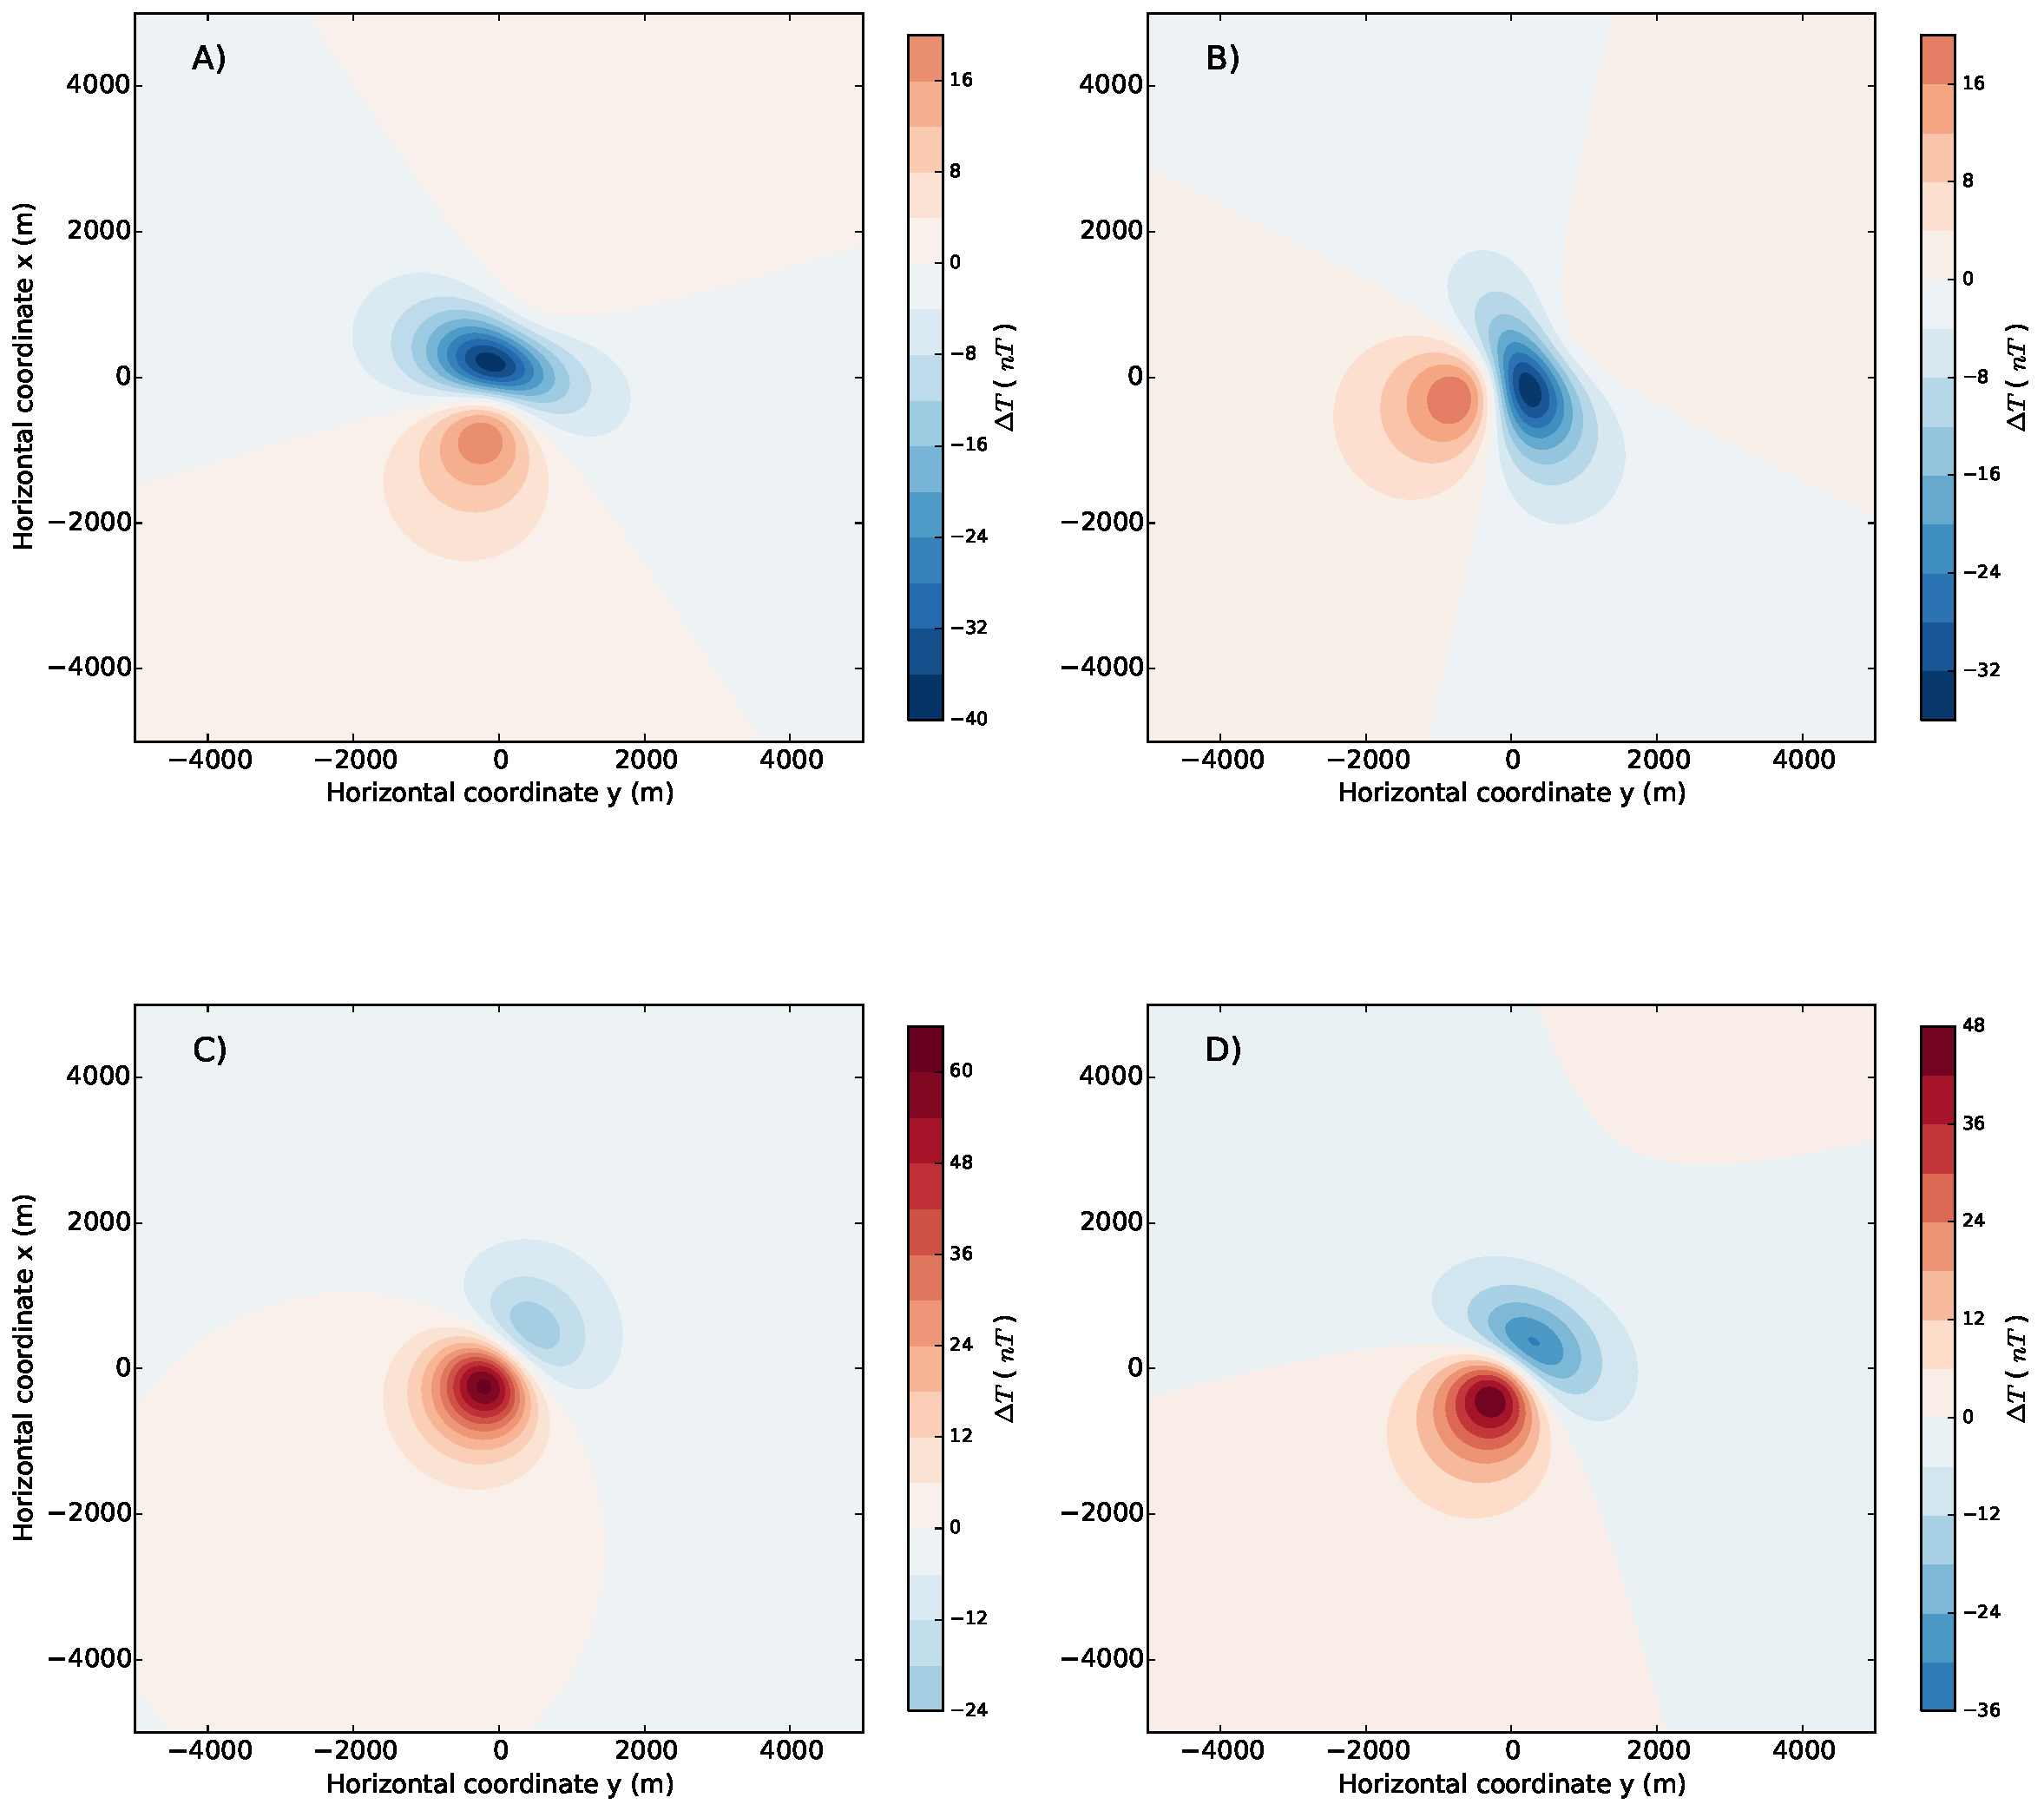
\includegraphics[width=16cm,height=16cm]{figures/ellipsoid_triaxial}
	\caption[Campo gerado pelo elipsoide triaxial definido na Tabela \ref{tab:triaxial}. A), B) e C) Componentes $x$, $y$ e $z$, respectivamente, da indução magnética $\Delta \mathbf{B}(\mathbf{r})$ (Eq. \ref{eq:delta-T-tilde}). D) Anomalia de campo total $\Delta T (\mathbf{r})$ (Eq. \ref{eq:delta-T-tilde-approx}). Todos os valores estão em nT.]{Campo gerado pelo elipsoide triaxial definido na Tabela \ref{tab:triaxial}. A), B) e C) Componentes $x$, $y$ e $z$, respectivamente, da indução magnética $\Delta \mathbf{B}(\mathbf{r})$ (Eq. \ref{eq:delta-T-tilde}). D) Anomalia de campo total $\Delta T (\mathbf{r})$ (Eq. \ref{eq:delta-T-tilde-approx}). Todos os valores estão em nT.}
	\label{fig:triaxial}
\end{figure}

As Figuras \ref{fig:prolate}A), \ref{fig:prolate}B), \ref{fig:prolate}C) e \ref{fig:prolate}D) mostram, respectivamente, as componentes $x$, $y$ e $z$ da indução magnética $\Delta \mathbf{B}(\mathbf{r})$ (Eq. \ref{eq:delta-T-tilde}) e a
anomalia de campo total $\Delta T (\mathbf{r})$ (Eq. \ref{eq:delta-T-tilde-approx}) produzidas pelo elipsoide prolato definido de acordo com os parâmetros da Tabela 4.2.

As Figuras \ref{fig:oblate}A), \ref{fig:oblate}B), \ref{fig:oblate}C) e \ref{fig:oblate}D) mostram, respectivamente, as componentes $x$, $y$ e $z$ da indução magnética $\Delta \mathbf{B}(\mathbf{r})$ (Eq. \ref{eq:delta-T-tilde}) e a
anomalia de campo total $\Delta T (\mathbf{r})$ (Eq. \ref{eq:delta-T-tilde-approx}) produzidas pelo elipsoide prolato definido de acordo com os parâmetros da Tabela 4.3.
\\\\\\

\begin{table}[h!]
	\begin{center}
		\begin{tabular}{|l|c|c|}
			\hline
			\textbf{Parâmetro}  & \textbf{Valor}  & \textbf{Unidade} \\
			\hline 
			$a$, $b$   & 200, 100 & m\\
			\hline
			\textit{strike}   & $45$ & º\\
			\hline
			\textit{dip}    & $0$ & º\\
			\hline
			\textit{rake}   & $0$  & º\\
			\hline
			$x_c$   & 0  & m\\
			\hline          
			$y_c$   & 0  & m\\
			\hline                
			$z_c$   & 1000  & m\\
			\hline
			$\mathbf{M}_{R}$*  & 100, $90$, $0$ & $A/m$, $^{\circ}$, $^{\circ}$\\
			\hline
			$B_0$*    & 60000, $50$, $20$ & $nT$, $^{\circ}$, $^{\circ}$\\
			\hline
			$k_{1}$, $k_{2}$, $k_{3}$   & 0.1, 0.1, 0.1  & SI, SI, SI\\
			\hline
			Orientação das colunas da matriz $\mathbf{U}$**   & $0$, $90$, $90$  & º, º, º\\
			\hline
			
		\end{tabular}
		\caption{Parâmetros do elipsoide triaxial modelado. *Valores de intensidade, inclinação e declinação respectivamente. **Ângulo de \textit{strike} , \textit{dip}  e \textit{rake} , respectivamente, para calcular os vetores unitários $\mathbf{u}_{1}$, $\mathbf{u}_{2}$, $\mathbf{u}_{3}$ por meio das Eqs. \ref{eq:v1_triaxial_prolate}, \ref{eq:v2_triaxial_prolate} e \ref{eq:v3_triaxial_prolate}.}
	\end{center}
	\label{tab:prolato}
\end{table}

\begin{table}[h!]
	\begin{center}
		\begin{tabular}{lc}
		
			 &  \\
			 & \\
			 & \\
			 & \\
			& \\
			& \\ 
			& \\
			& \\
			& \\ 
			& \\
\end{tabular}
\end{center}
\end{table}

\begin{table}[h!]
	\begin{center}
		\begin{tabular}{|l|c|c|}
			\hline
			\textbf{Parâmetro}  & \textbf{Valor} & \textbf{Unidade} \\
			\hline 
			$a$, $b$  & 100, 200 & m \\
			\hline
			\textit{strike}   & $45$ & º\\
			\hline
			\textit{dip}    & $0$ & º\\
			\hline
			\textit{rake}   & $0$  & º\\
			\hline
			$x_c $  & 0  & m\\
			\hline          
			$y_c$   & 0  & m\\
			\hline                
			$z_c$   & 1000  & m\\
			\hline
			$\mathbf{M}_{R}$*  & 100, $90$, $0$  & $A/m$, $^{\circ}$, $^{\circ}$\\
			\hline
			$B_0$*    & 60000, $50$, $20$ & $nT$, $^{\circ}$, $^{\circ}$\\
			\hline
			$k_{1}$, $k_{2}$, $k_{3}$   & 0.1, 0.1, 0.1  & SI, SI, SI\\
			\hline
			Orientação das colunas da matriz $\mathbf{U}$**   & $0$, $90$, $90$  & º, º, º\\
			\hline
		\end{tabular}
		\caption{Parâmetros do elipsoide triaxial modelado. *Valores de intensidade, inclinação e declinação respectivamente. **Ângulo de \textit{strike} , \textit{dip}  e \textit{rake} , respectivamente, para calcular os vetores unitários $\mathbf{u}_{1}$, $\mathbf{u}_{2}$, $\mathbf{u}_{3}$ por meio das Eqs. \ref{eq:v1_triaxial_prolate}, \ref{eq:v2_triaxial_prolate} e \ref{eq:v3_triaxial_prolate}.}
	\end{center}
	\label{tab:oblate}
\end{table}

\begin{figure}[hbt!]
	\centering 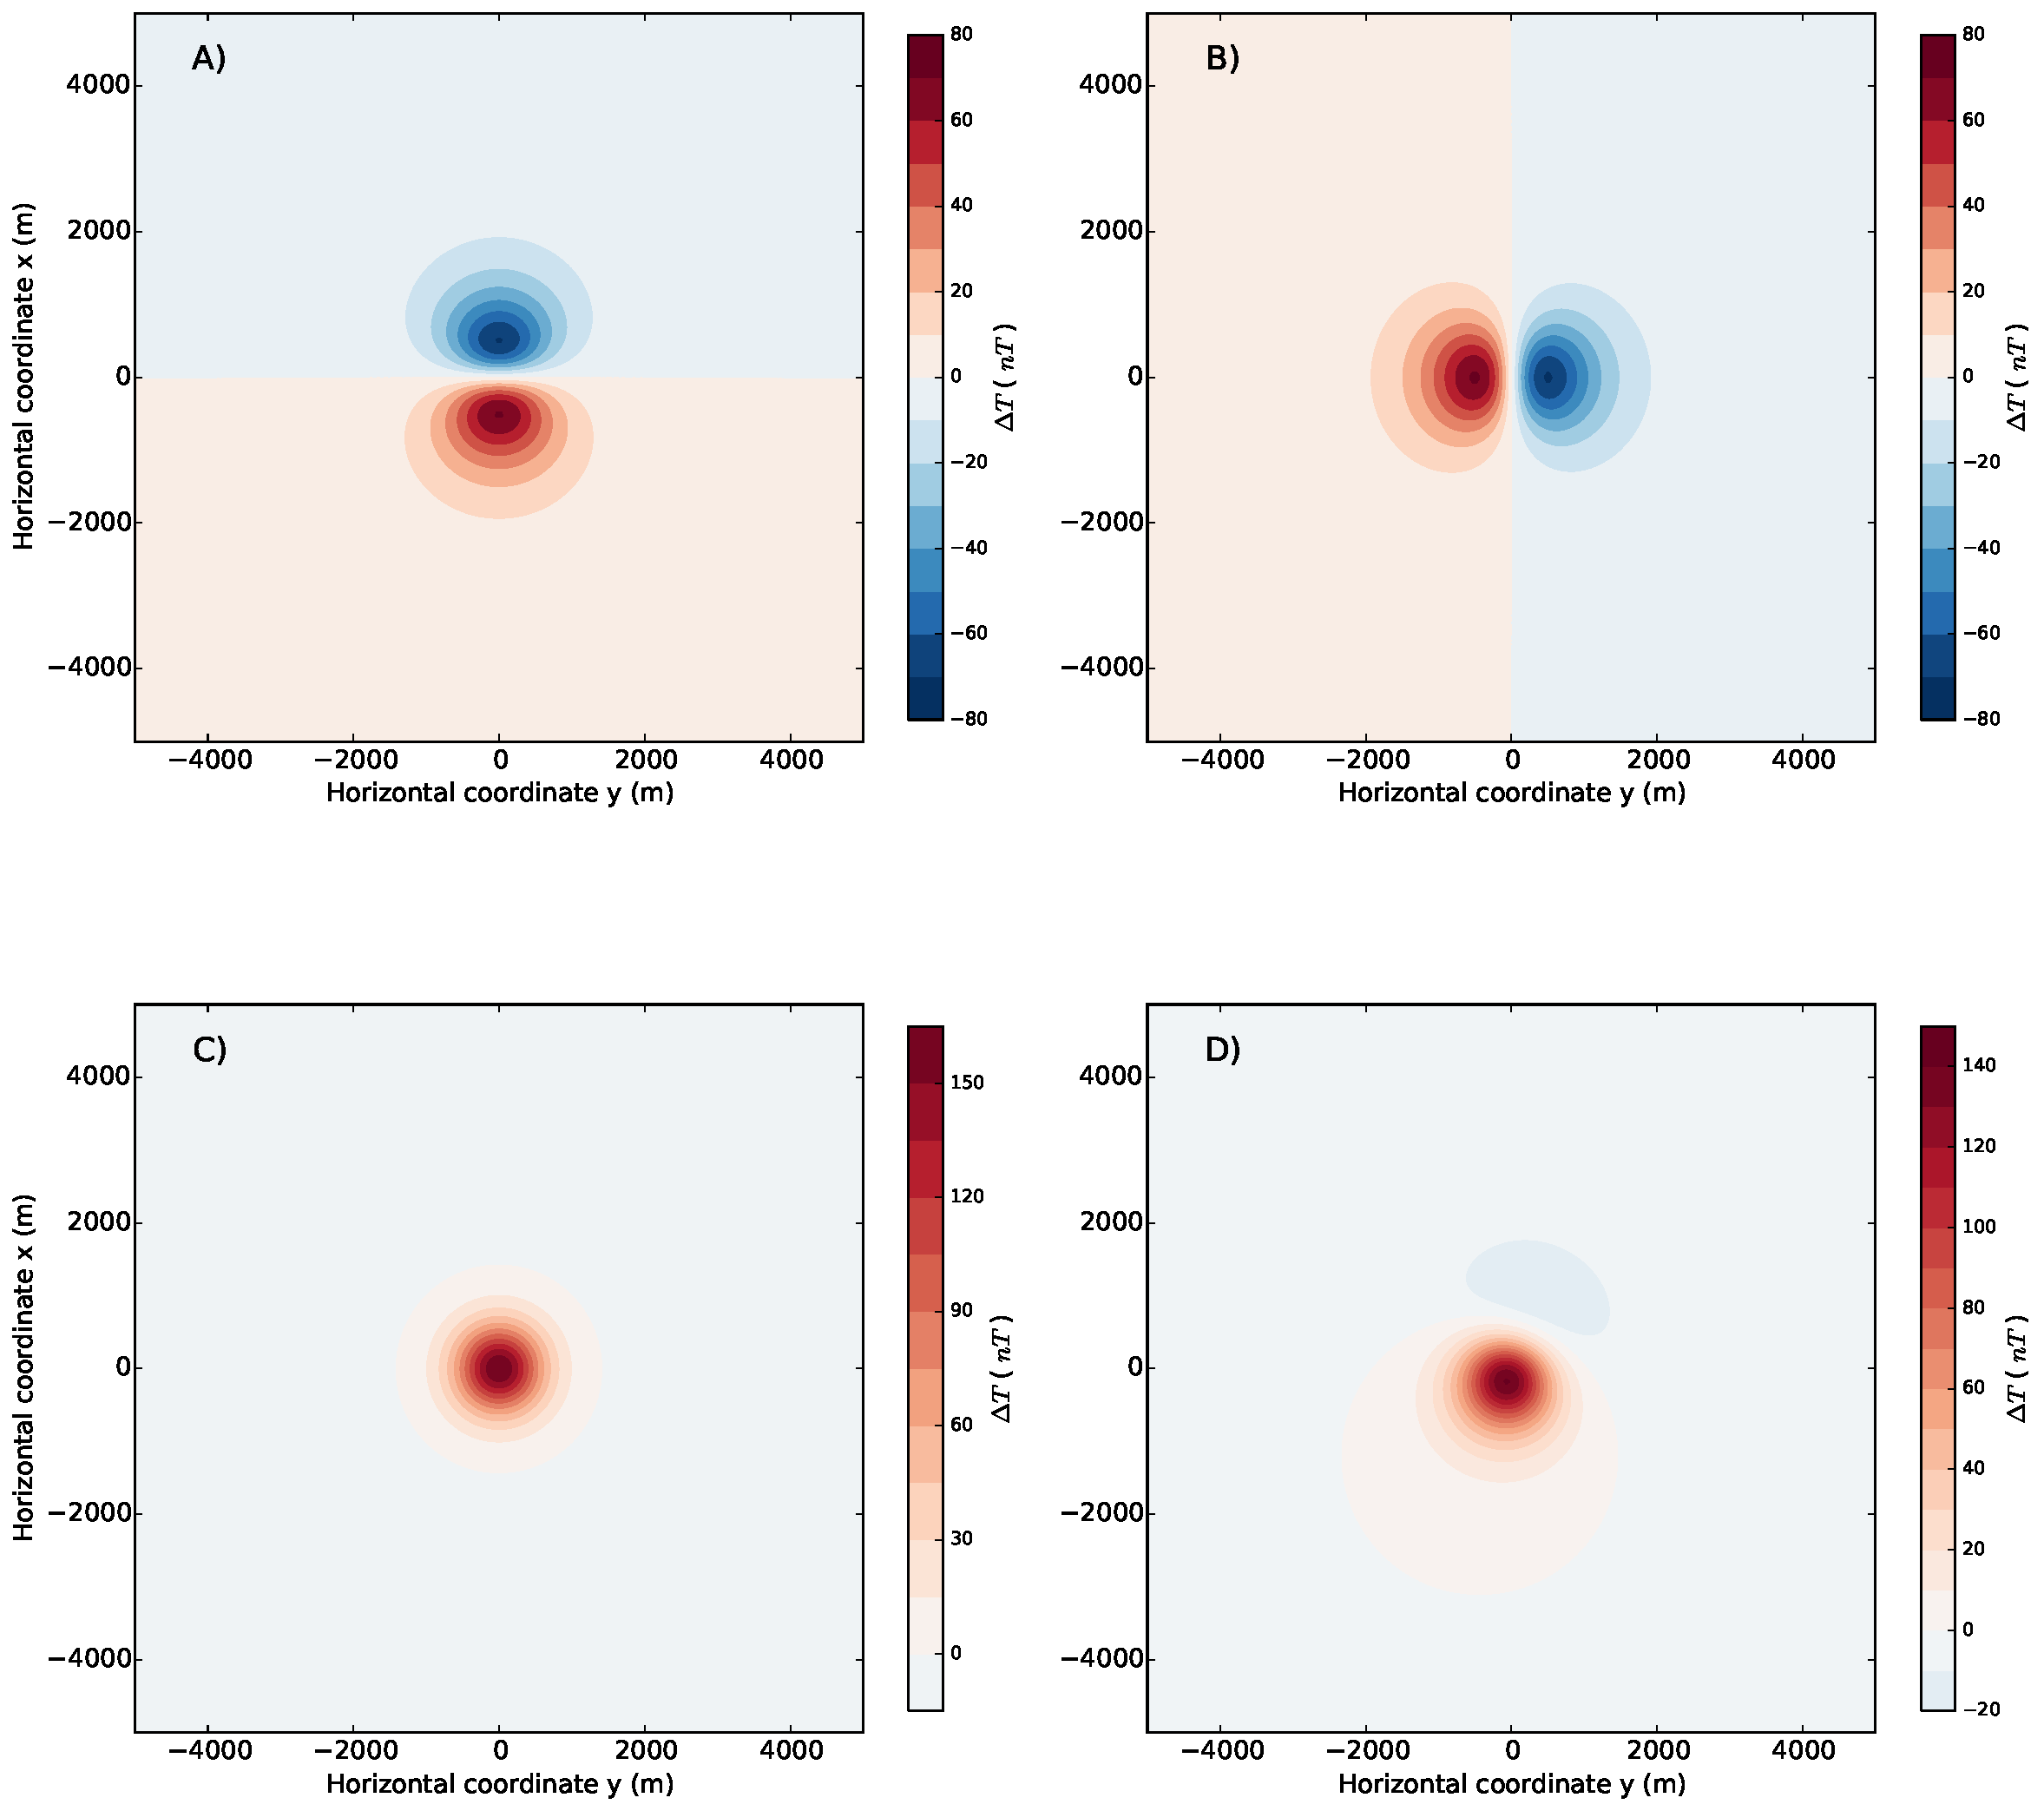
\includegraphics[width=16cm,height=16cm]{figures/ellipsoid_prolate}
	\caption[As componentes do campo magnético gerado por um elipsoide prolato e a anomalia de campo total aproximada.]{As componentes 
		do campo magnético gerado por um elipsoide prolato de parâmetros conforme a tabela 4.2 e a anomalia de campo total aproximada. Em A) a componente Bx do campo, em B) a componente By, em C) a componente Bz e em D) a anomalia de campo total aproximada.}
	\label{fig:prolate}
\end{figure}

\begin{table}[h!]
	\begin{center}
		\begin{tabular}{lc}
			
			&  \\
			& \\
			& \\
			& \\
			& \\
			& \\ 
			& \\
			& \\
		\end{tabular}
	\end{center}
\end{table}

\begin{figure}[hbt!]
	\centering 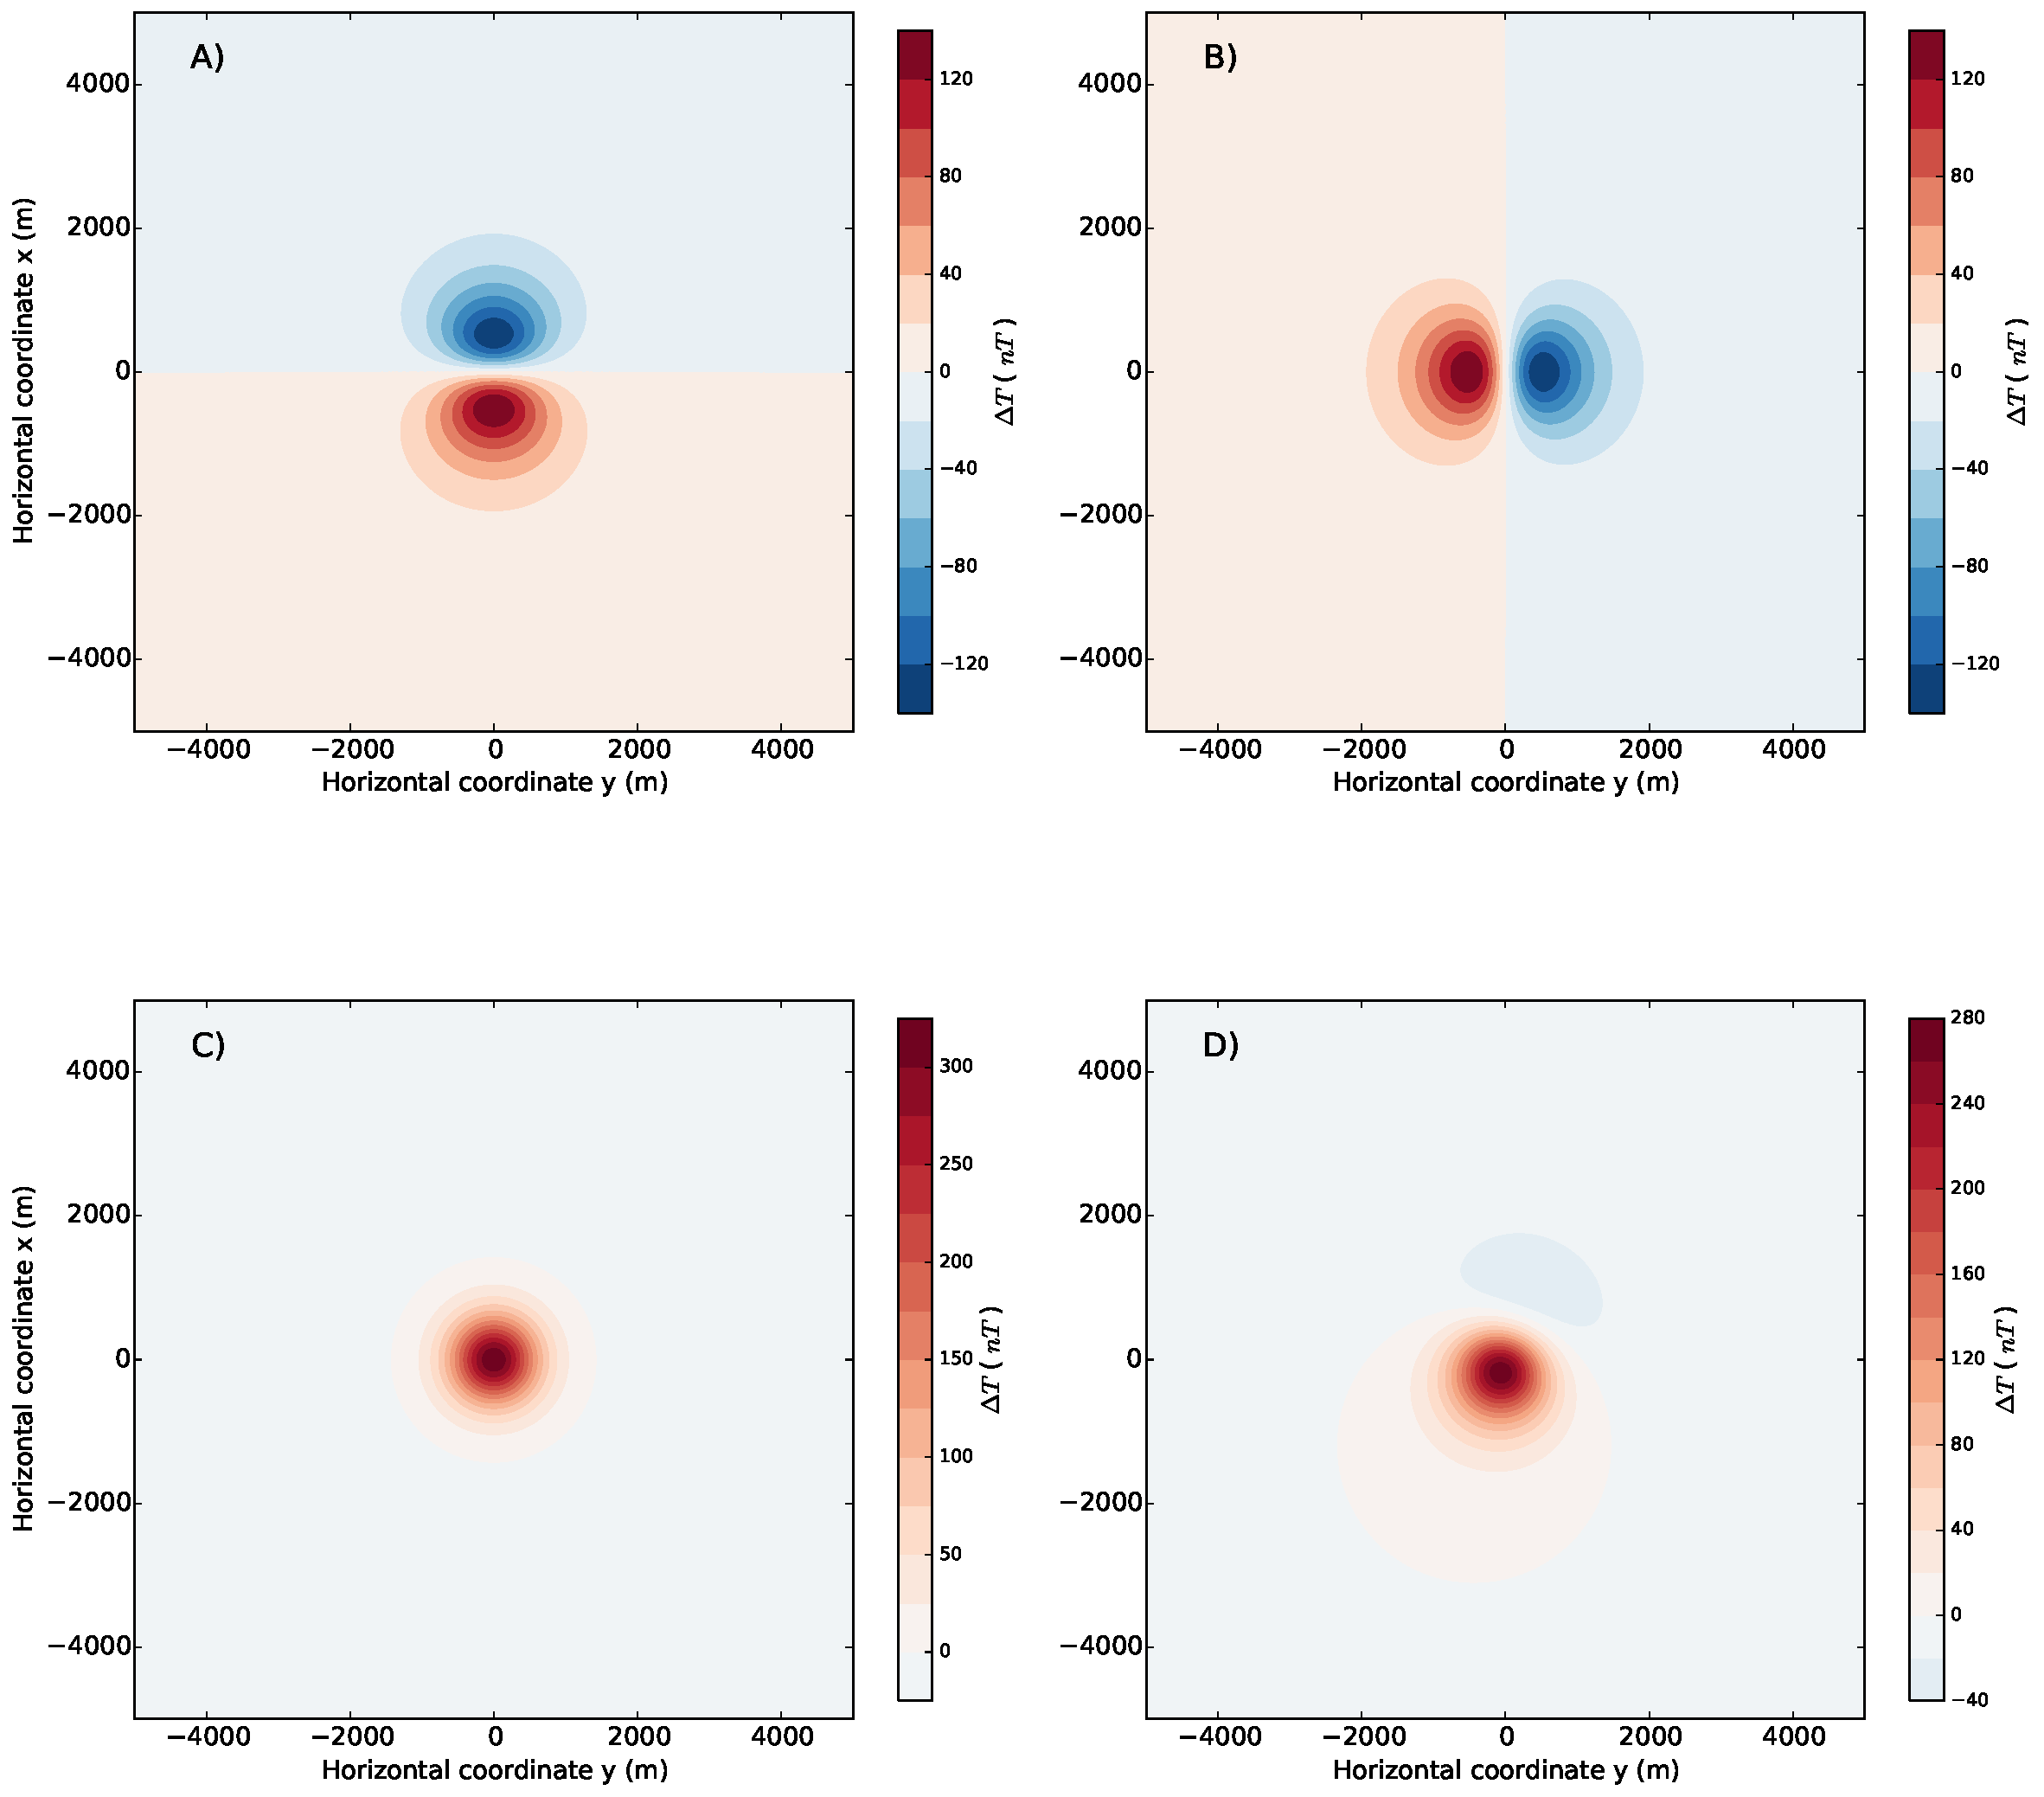
\includegraphics[width=16cm,height=16cm]{figures/ellipsoid_oblate}
	\caption[As componentes do campo magnético gerado por um elipsoide oblato e a anomalia de campo total aproximada.]{As componentes 
		do campo magnético gerado por um elipsoide oblato de parâmetros conforme a tabela 4.3 e a anomalia de campo total aproximada. Em A) a componente Bx do campo, em B) a componente By, em C) a componente Bz e em D) a anomalia de campo total aproximada.}
	\label{fig:oblate}
\end{figure}

As Figuras \ref{fig:ellipsoid_triaxial_multi}A), \ref{fig:ellipsoid_triaxial_multi}B), \ref{fig:ellipsoid_triaxial_multi}C) e \ref{fig:ellipsoid_triaxial_multi}D) mostram, respectivamente, as componentes $x$, $y$ e $z$ da indução magnética $\Delta \mathbf{B}(\mathbf{r})$ (Eq. \ref{eq:delta-T-tilde}) e a
anomalia de campo total $\Delta T (\mathbf{r})$ (Eq. \ref{eq:delta-T-tilde-approx}) produzidas por dois elipsoides triaxiais definidos de acordo com os parâmetros da Tabela 4.4.

\begin{table}[h!]
	\begin{center}
		\begin{tabular}{lc}
			
			&  \\
			&  \\
			&  \\
			&  \\
		\end{tabular}
	\end{center}
\end{table}

\begin{table}[h!]
	\begin{center}
		\begin{tabular}{|l|c|c|}
			\hline
			\textbf{Parâmetro}  & \textbf{Valor}  & \textbf{Unidade}\\
			\hline 
			$a$, $b$, $c$   & 150, 100, 75 & m\\
			\hline
			\textit{strike}   & $0$ & º\\
			\hline
			\textit{dip}    & $0$ & º\\
			\hline
			\textit{rake}   & $0$  & º\\
			\hline
			$x_c$   & -2500  & m\\
			\hline          
			$y_c$   & -2500  & m\\
			\hline                
			$z_c$  & 1000  & m\\
			\hline
			$\mathbf{M}_{R}$*  & 100, $25^o$, $40^o$  & $A/m$, $^{\circ}$, $^{\circ}$\\
			\hline
			$k_1$, $k_2$, $k_3$   & 0.1, 0.1, 0.1  & SI, SI, SI\\
			\hline
			Orientação das colunas da matriz $\mathbf{U}$**   & $0$, $90$, $90$  & º, º, º\\
			\hline 
			a$_2$, b$_2$, c$_2$   & 200, 120, 60 & m\\
			\hline
			\textit{strike}$_2$   & $0$ & º\\
			\hline
			\textit{dip}$_2$    & $0$ & º\\
			\hline
			\textit{rake}$_2$   & $0$  & º\\
			\hline
			$x_{c2}$   & 2500  & m\\
			\hline          
			$y_{c2}$   & 2500  & m\\
			\hline                
			$z_{c2}$   & 1000  & m\\
			\hline
			$\mathbf{M}_{R2}$*  & 75, $25^o$, $40^o$  & $A/m$, $^{\circ}$, $^{\circ}$\\
			\hline
			$k_12$, $k_22$, $k_32$   & 0.1, 0.1, 0.1  & SI, SI, SI\\
			\hline
			Orientação das colunas da matriz $\mathbf{U}_2$**   & $0$, $90$, $90$  & º, º, º\\
			\hline
			$B_0$*    & 60000, $50^o$, $20^o$ & $nT$, $^{\circ}$, $^{\circ}$\\
			\hline			
		\end{tabular}
		\caption{Parâmetros dos elipsoides triaxiais modelados. *Valores de intensidade, inclinação e declinação respectivamente. **Ângulo de \textit{strike} , \textit{dip}  e \textit{rake} , respectivamente, para calcular os vetores unitários $\mathbf{u}_{1}$, $\mathbf{u}_{2}$, $\mathbf{u}_{3}$ por meio das Eqs. \ref{eq:v1_triaxial_prolate}, \ref{eq:v2_triaxial_prolate} e \ref{eq:v3_triaxial_prolate}.}
	\end{center}
	\label{tab:ellipsoid_triaxial_multi}
\end{table}

\begin{table}[h!]
	\begin{center}
		\begin{tabular}{lc}
			
			&  \\
			& \\
			& \\
			& \\
			& \\
			& \\ 
			& \\
			& \\
				& \\
				& \\ 
				& \\
		\end{tabular}
	\end{center}
\end{table}

\begin{figure}[hbt!]
	\centering 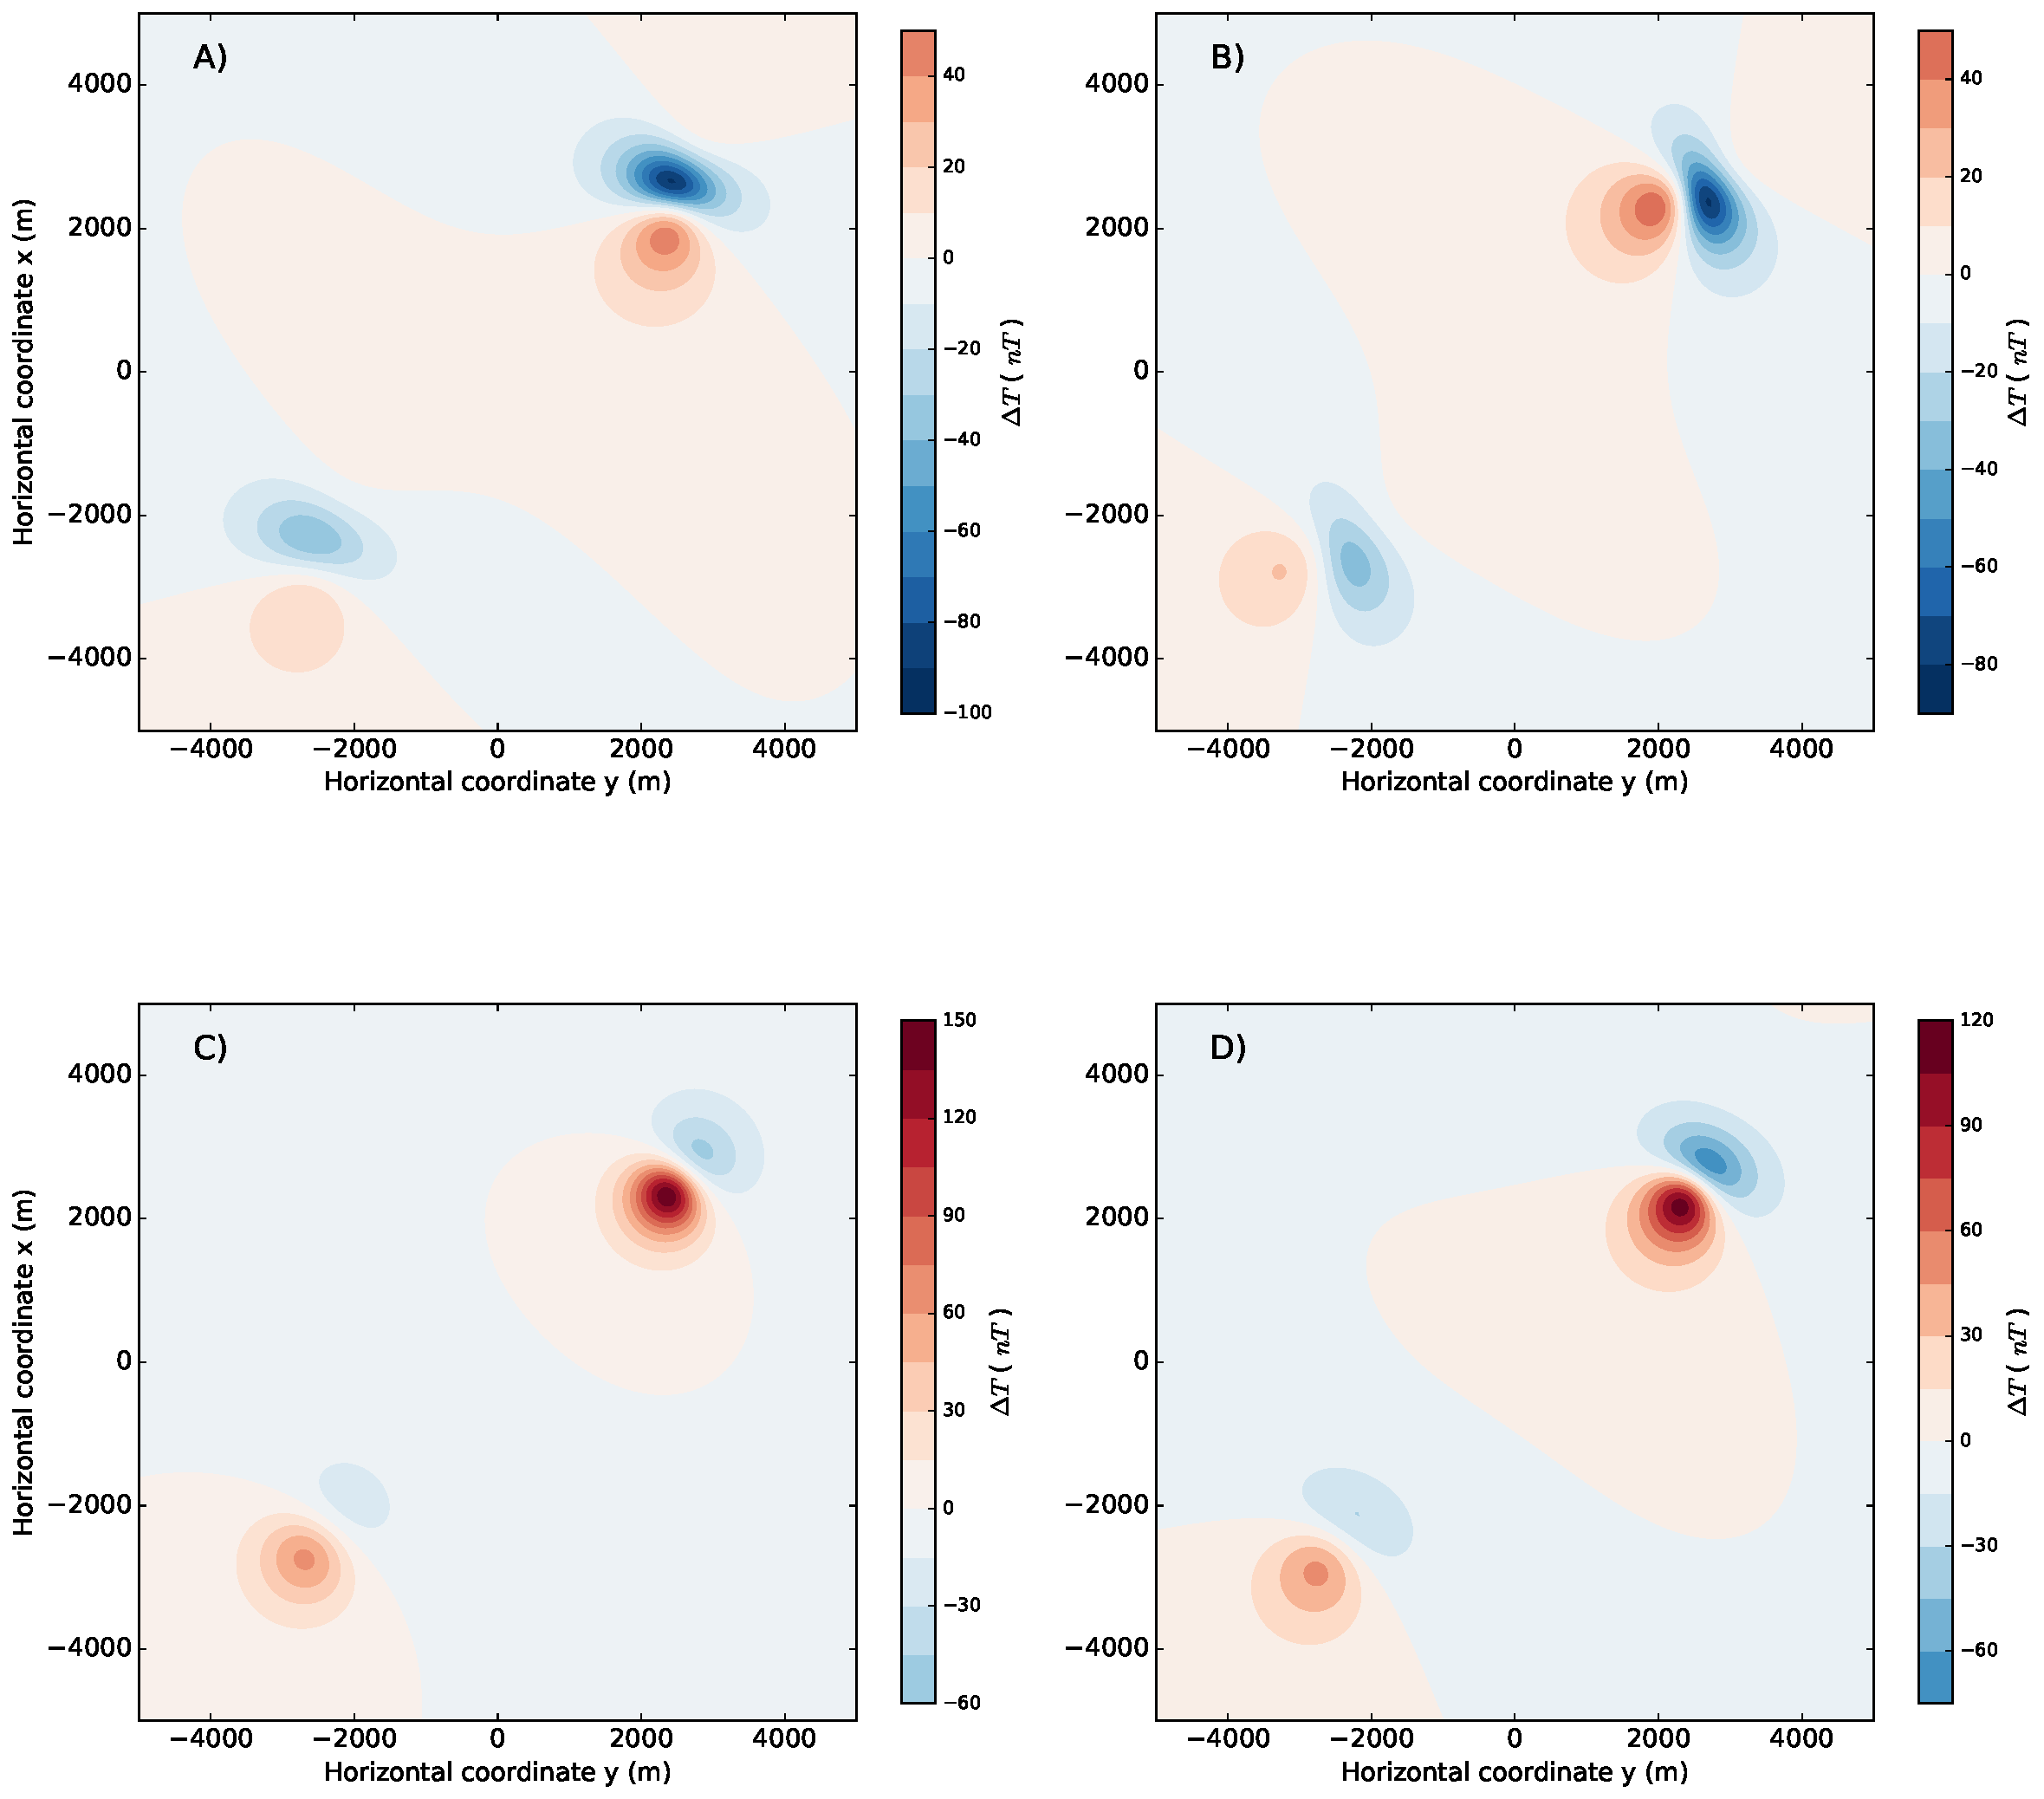
\includegraphics[width=16cm,height=16cm]{figures/ellipsoid_triaxial_multi}
	\caption[As componentes do campo magnético gerado por dois corpos triaxiais e a anomalia de campo total aproximada.]{As componentes 
		do campo magnético gerado pelos elipsoides triaxiais de parâmetros conforme a tabela 4.4 e a anomalia de campo total aproximada. Em A) a componente Bx do campo, em B) a componente By, em C) a componente Bz e em D) a anomalia de campo total aproximada.}
	\label{fig:ellipsoid_triaxial_multi}
\end{figure}


\begin{figure}[hbt!]
	\centering 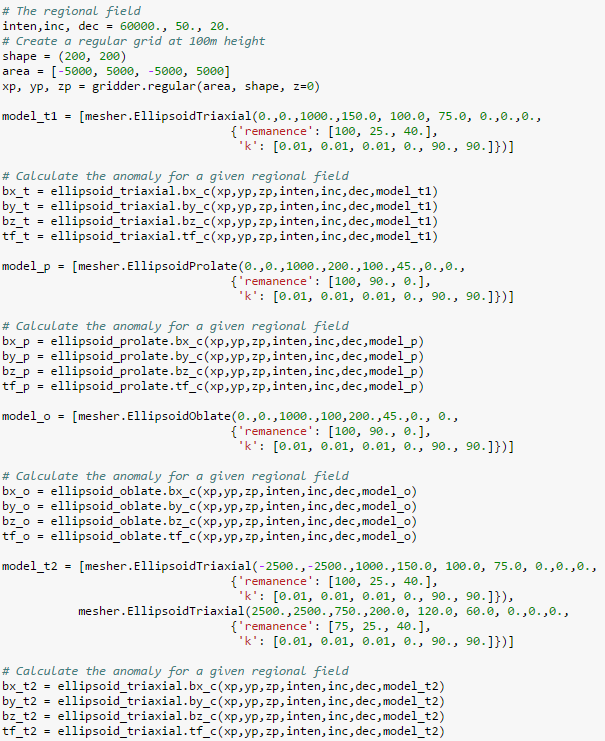
\includegraphics[width=16 cm,height=20 cm]{figures/mag_fields_0}
	\caption[As componentes do campo magnético gerado por dois corpos triaxiais e a anomalia de campo total aproximada.]{\textit{Scripts} utilizados para gerar os resultados mostrados na Figuras \ref{fig:triaxial}, \ref{fig:prolate}, \ref{fig:oblate} e \ref{fig:ellipsoid_triaxial_multi}. A descrição do código é similar àquela mostrada na Figura \ref{fig:Cookbook_Triaxial}.}
	\label{fig:mag_fields_0}
\end{figure}

\begin{table}[h!]
	\begin{center}
		\begin{tabular}{lc}
			
			&  \\
			& \\
			& \\
			& \\
			& \\
			& \\ 
			& \\
			& \\
		\end{tabular}
	\end{center}
\end{table}

\section{Elementos do tensor de depolarização}

Os fatores de desmagnetização são importantíssimos para a modelagem de corpos com alta susceptibilidade e dependem apenas da sua forma geométrica, no modelo elipsoidal. 

Na Figura \ref{fig:n_triaxial} observamos o comportamento afastado destes elementos, quando os semi-eixos de elipsoide triaxial possuem tamanhos diferentes, e a tendência de se aproximarem para um mesmo valor quando possuem tamanhos próximos (se aproximando de uma esfera, que possui o valor de $1/3$ no SI para todos os elementos dos fatores de desmagnetização).


\begin{figure}[hbt!]
	\centering 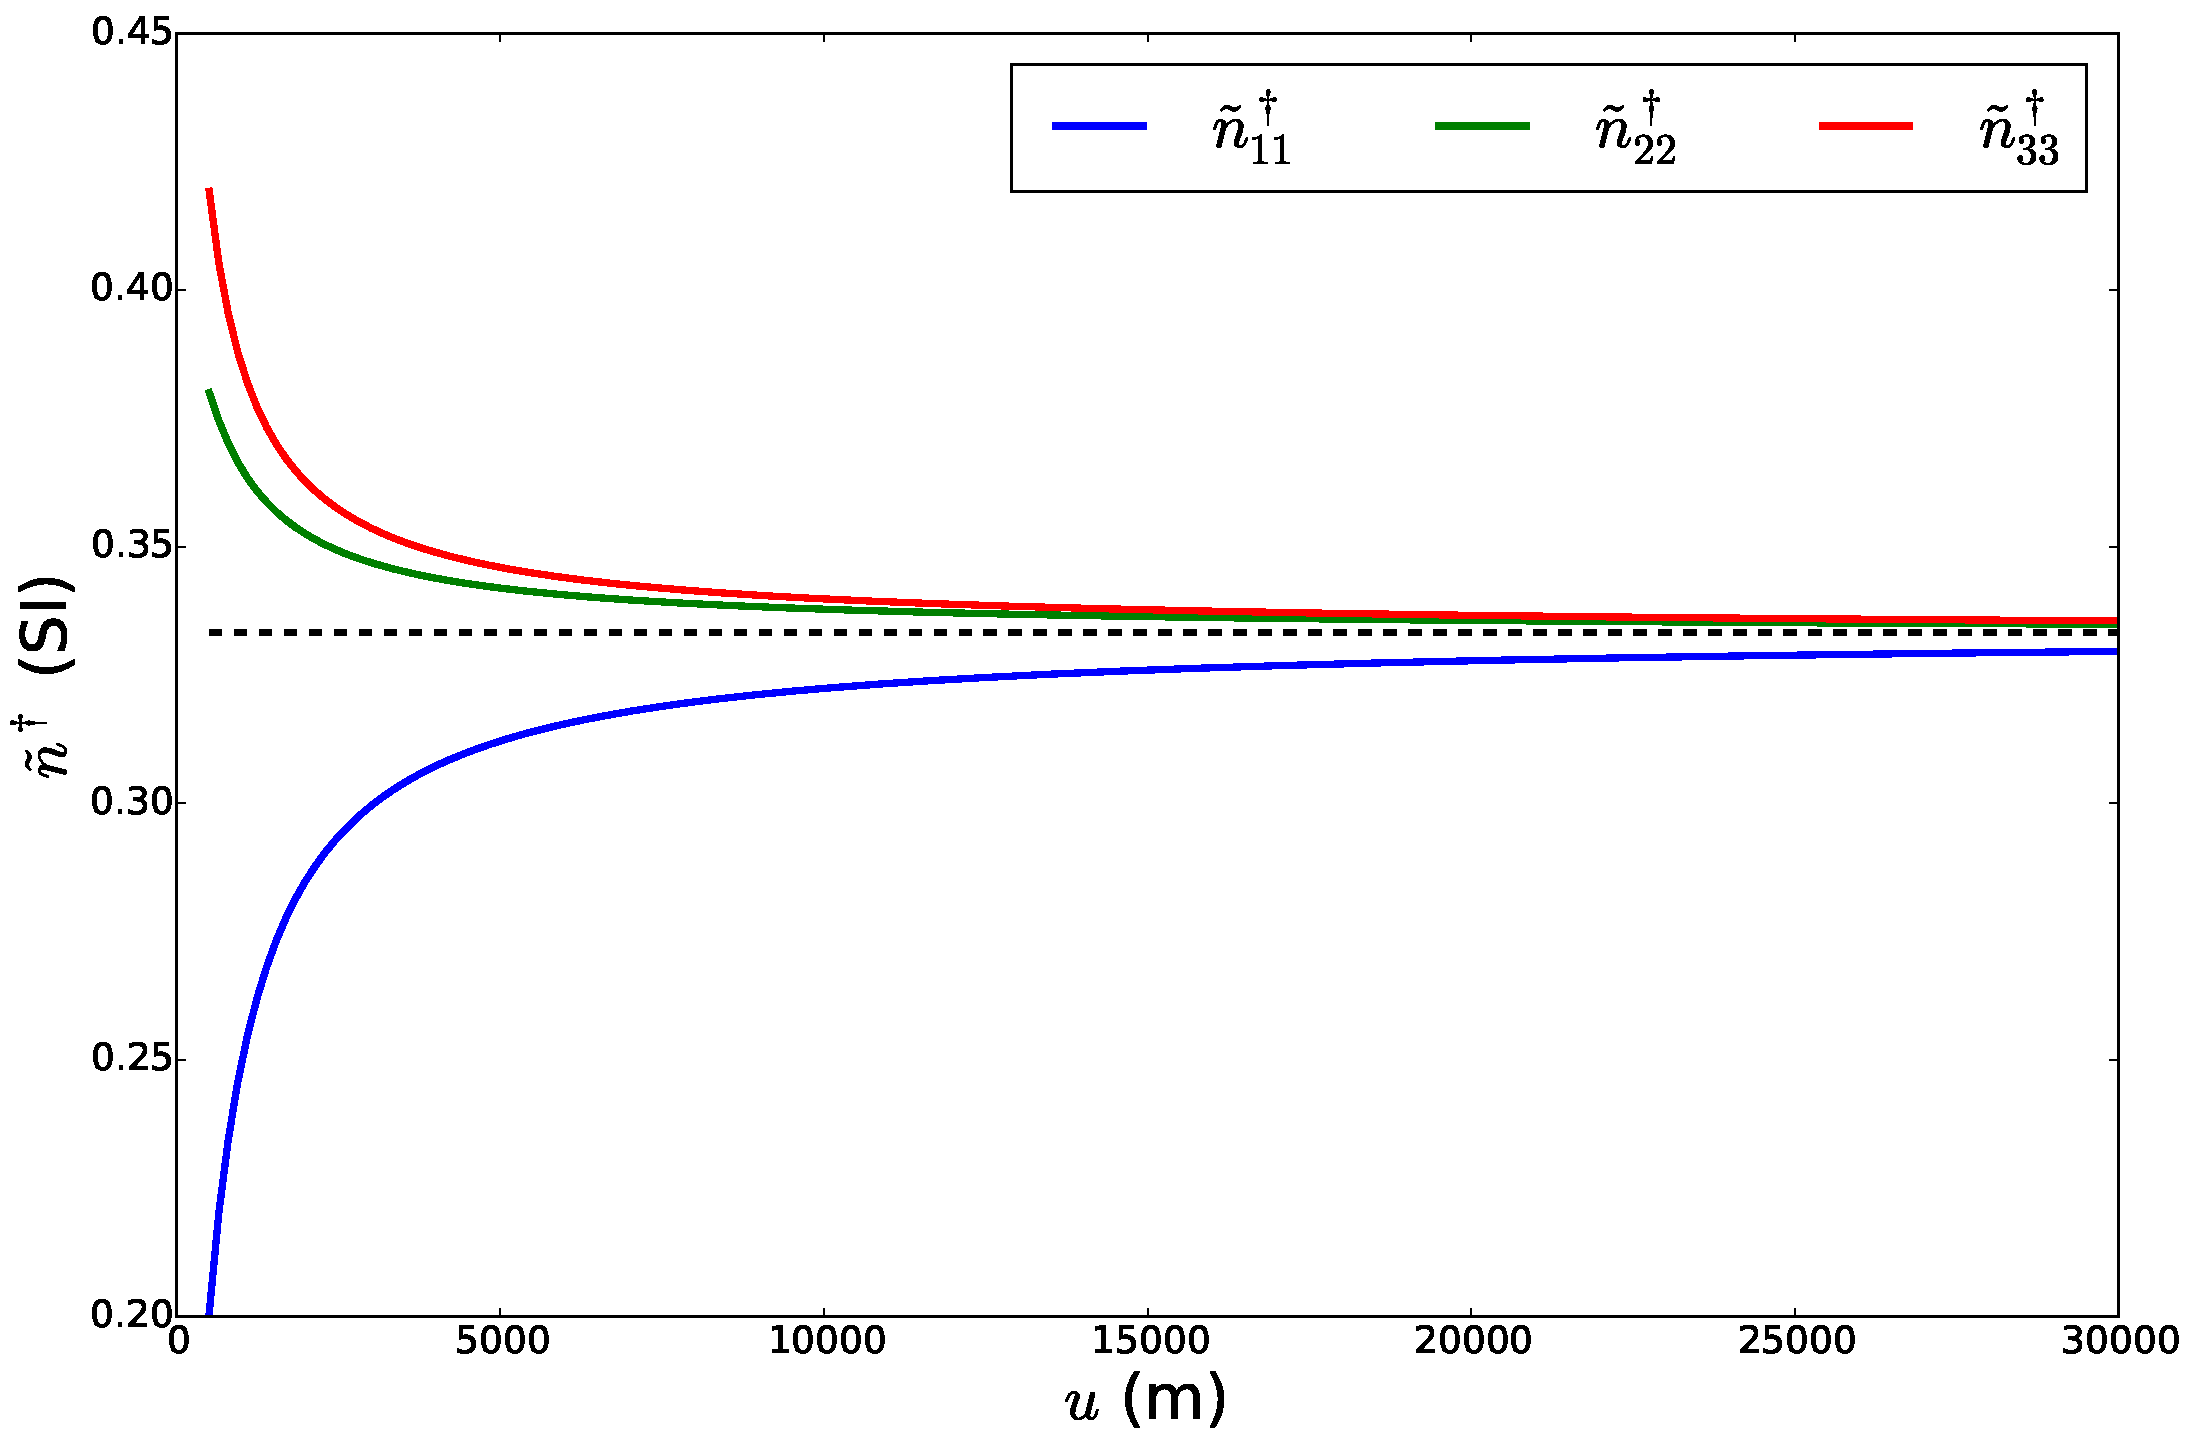
\includegraphics[width=15cm,height=10cm]{figures/test_n_triaxial}
	\caption[Teste dos fatores de desmagnetização para um elipsoide triaxial.]{Teste dos fatores de desmagnetização:
		$\tilde{n}^{\dagger}_{11}$, $\tilde{n}^{\dagger}_{22}$ e $\tilde{n}^{\dagger}_{33}$ 
		para um elipsoide triaxial originalmente com semi-eixos 500, 100 e 50 metros, com um fator $u$ crescente,
		somando, simultaneamente, todos os semi-eixos.}
	\label{fig:n_triaxial}
\end{figure}

Na Figura \ref{fig:n_prolato} observamos o mesmo comportamento no caso triaxial para o caso do elipsoide prolato. Neste gráfico no eixo horizontal é feita a relação entre os semi-eixos $a$ e $b$ ($m$) onde aumenta-se a valor do semi-eixo maior e mantém o semi-eixo menor constante. No começo, quando os semi-eixos estão próximos, os elementos tendem à $1/3$ e se afastam conforme $a$ é muito maior que $b$.
\newpage

\begin{figure}[hbt!]
	\centering 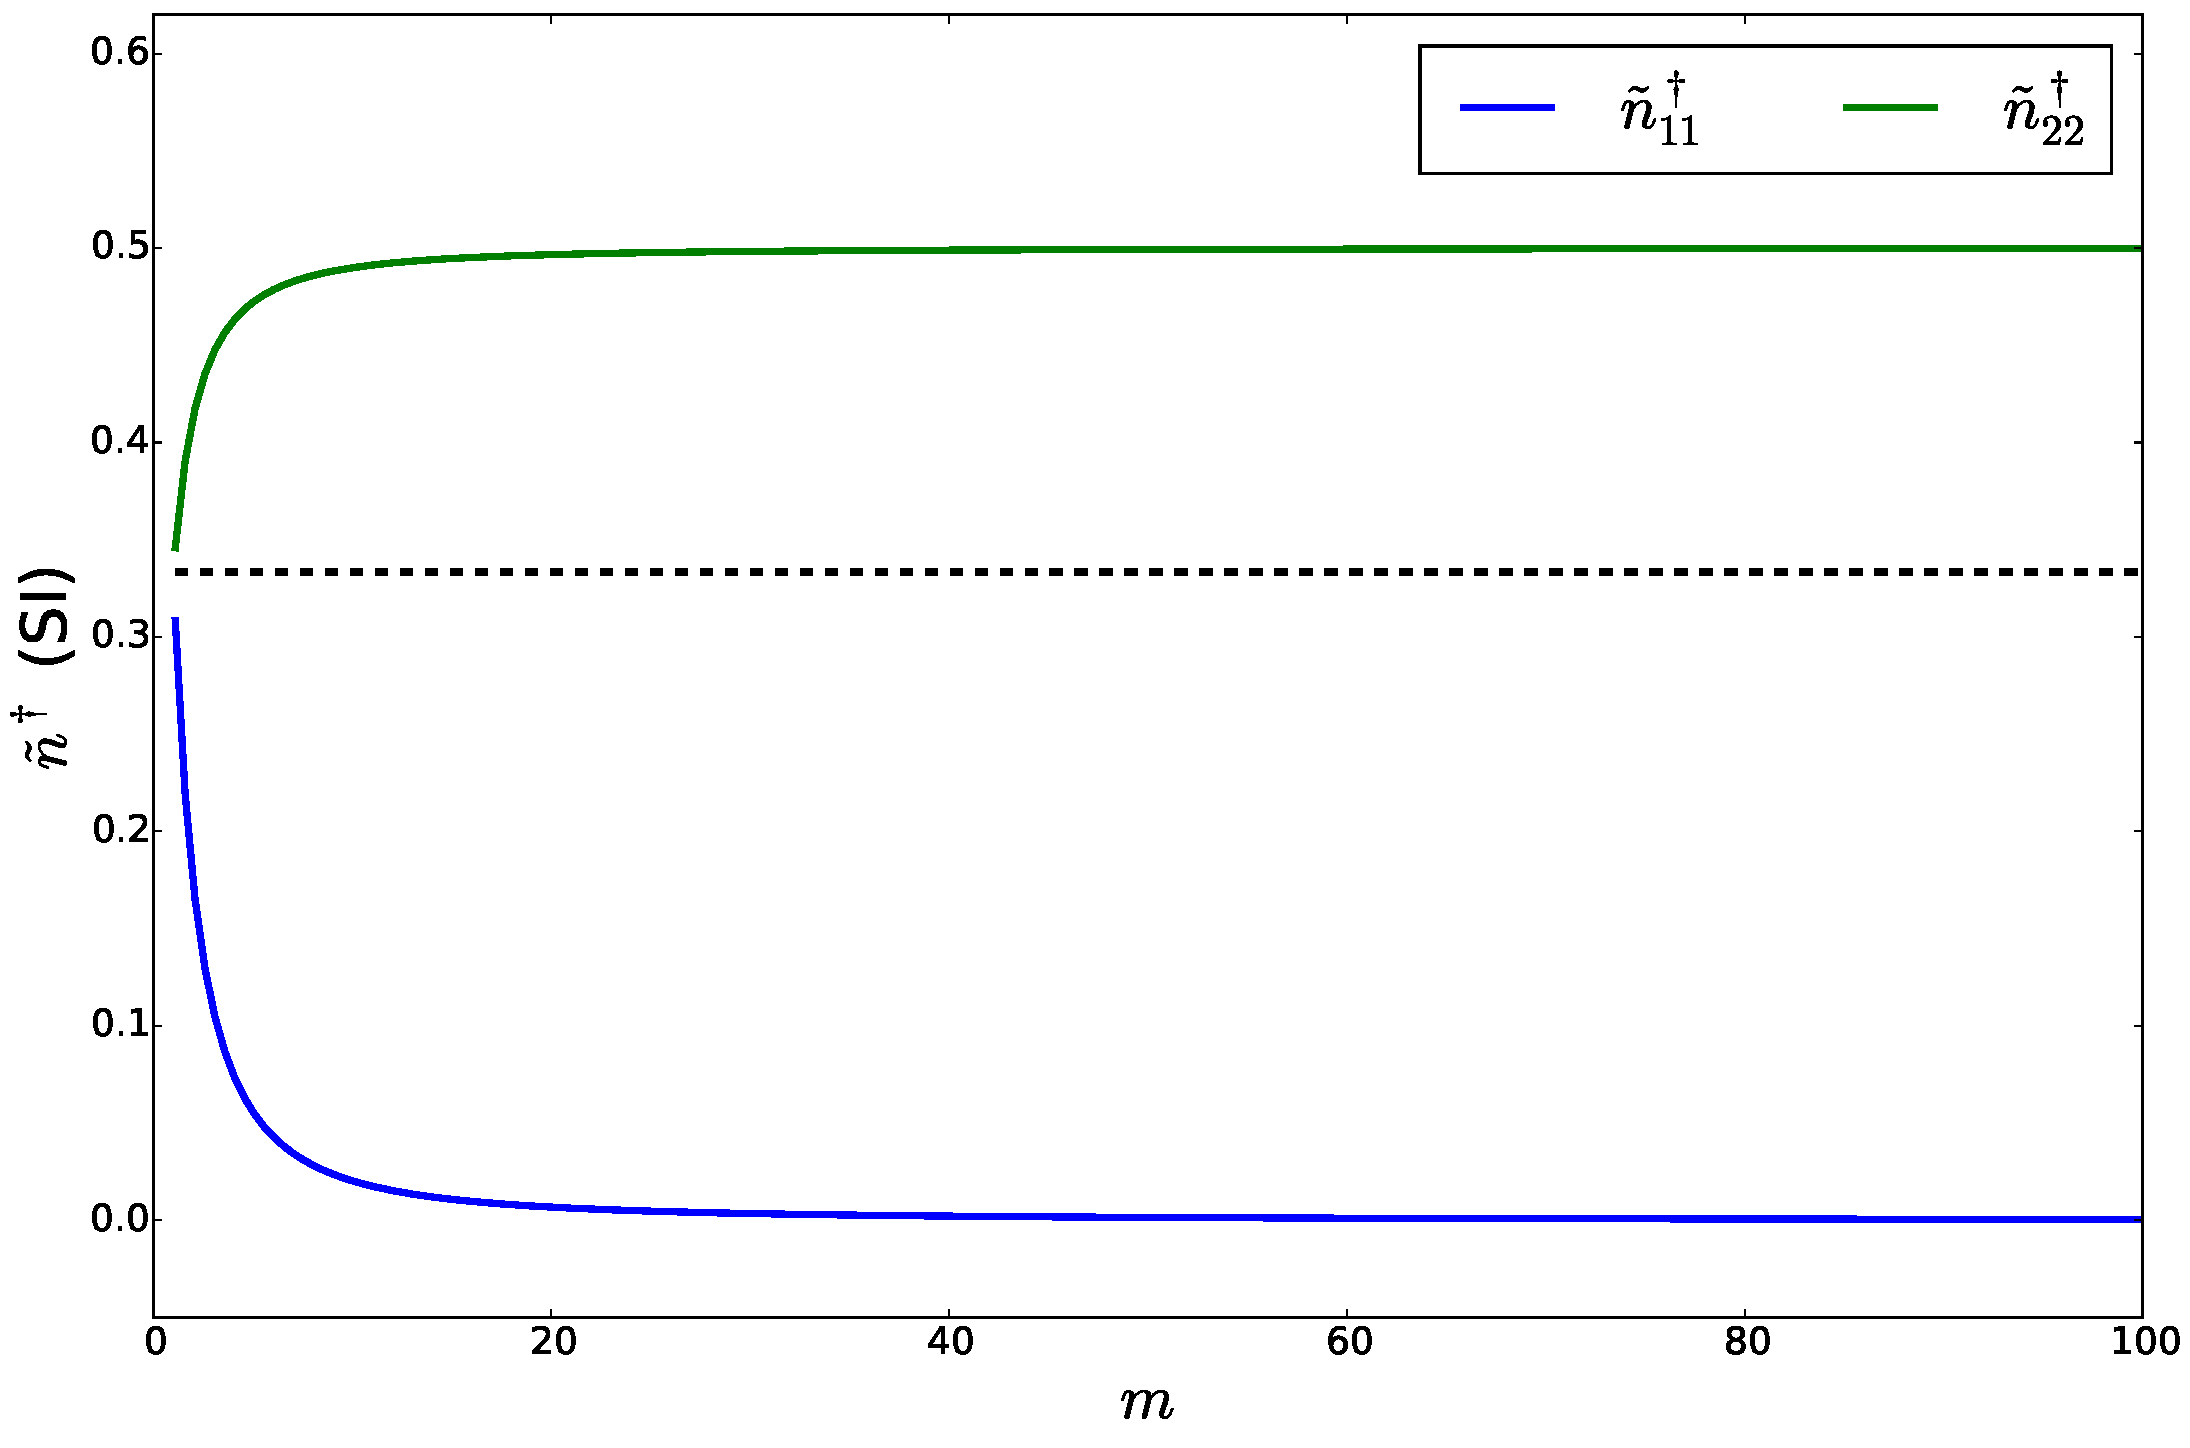
\includegraphics[width=15cm,height=10cm]{figures/test_n_prolate}
	\caption[Teste dos fatores de desmagnetização para um elipsoide prolato.]{Teste dos fatores de desmagnetização:
		$\tilde{n}^{\dagger}_{11}$ e $\tilde{n}^{\dagger}_{22}$
		para um elipsoide prolato originalmente com semi-eixos 110 e 100 metros, com um fator $m (a/b)$ crescente,
		aumentando a valor do semi-eixo maior e mantendo o semi-eixo menor constante.}
	\label{fig:n_prolato}
\end{figure}

Já na figura \ref{fig:n_oblato}realizamos a mesma relação entre os semi-eixos $a$ e $b$ do caso prolato, onde aumenta-se o valor de $a$. Lembremos que no caso do elipsoide oblato $a$ é o semi-eixo menor e $b$ o semi-eixo maior. No começo, quando os semi-eixos estão afastados, os elementos estão afastados para $b$ muito maior que $a$ e tendem à $1/3$ conforme se aproximam.
\newpage

\begin{figure}[hbt!]
	\centering 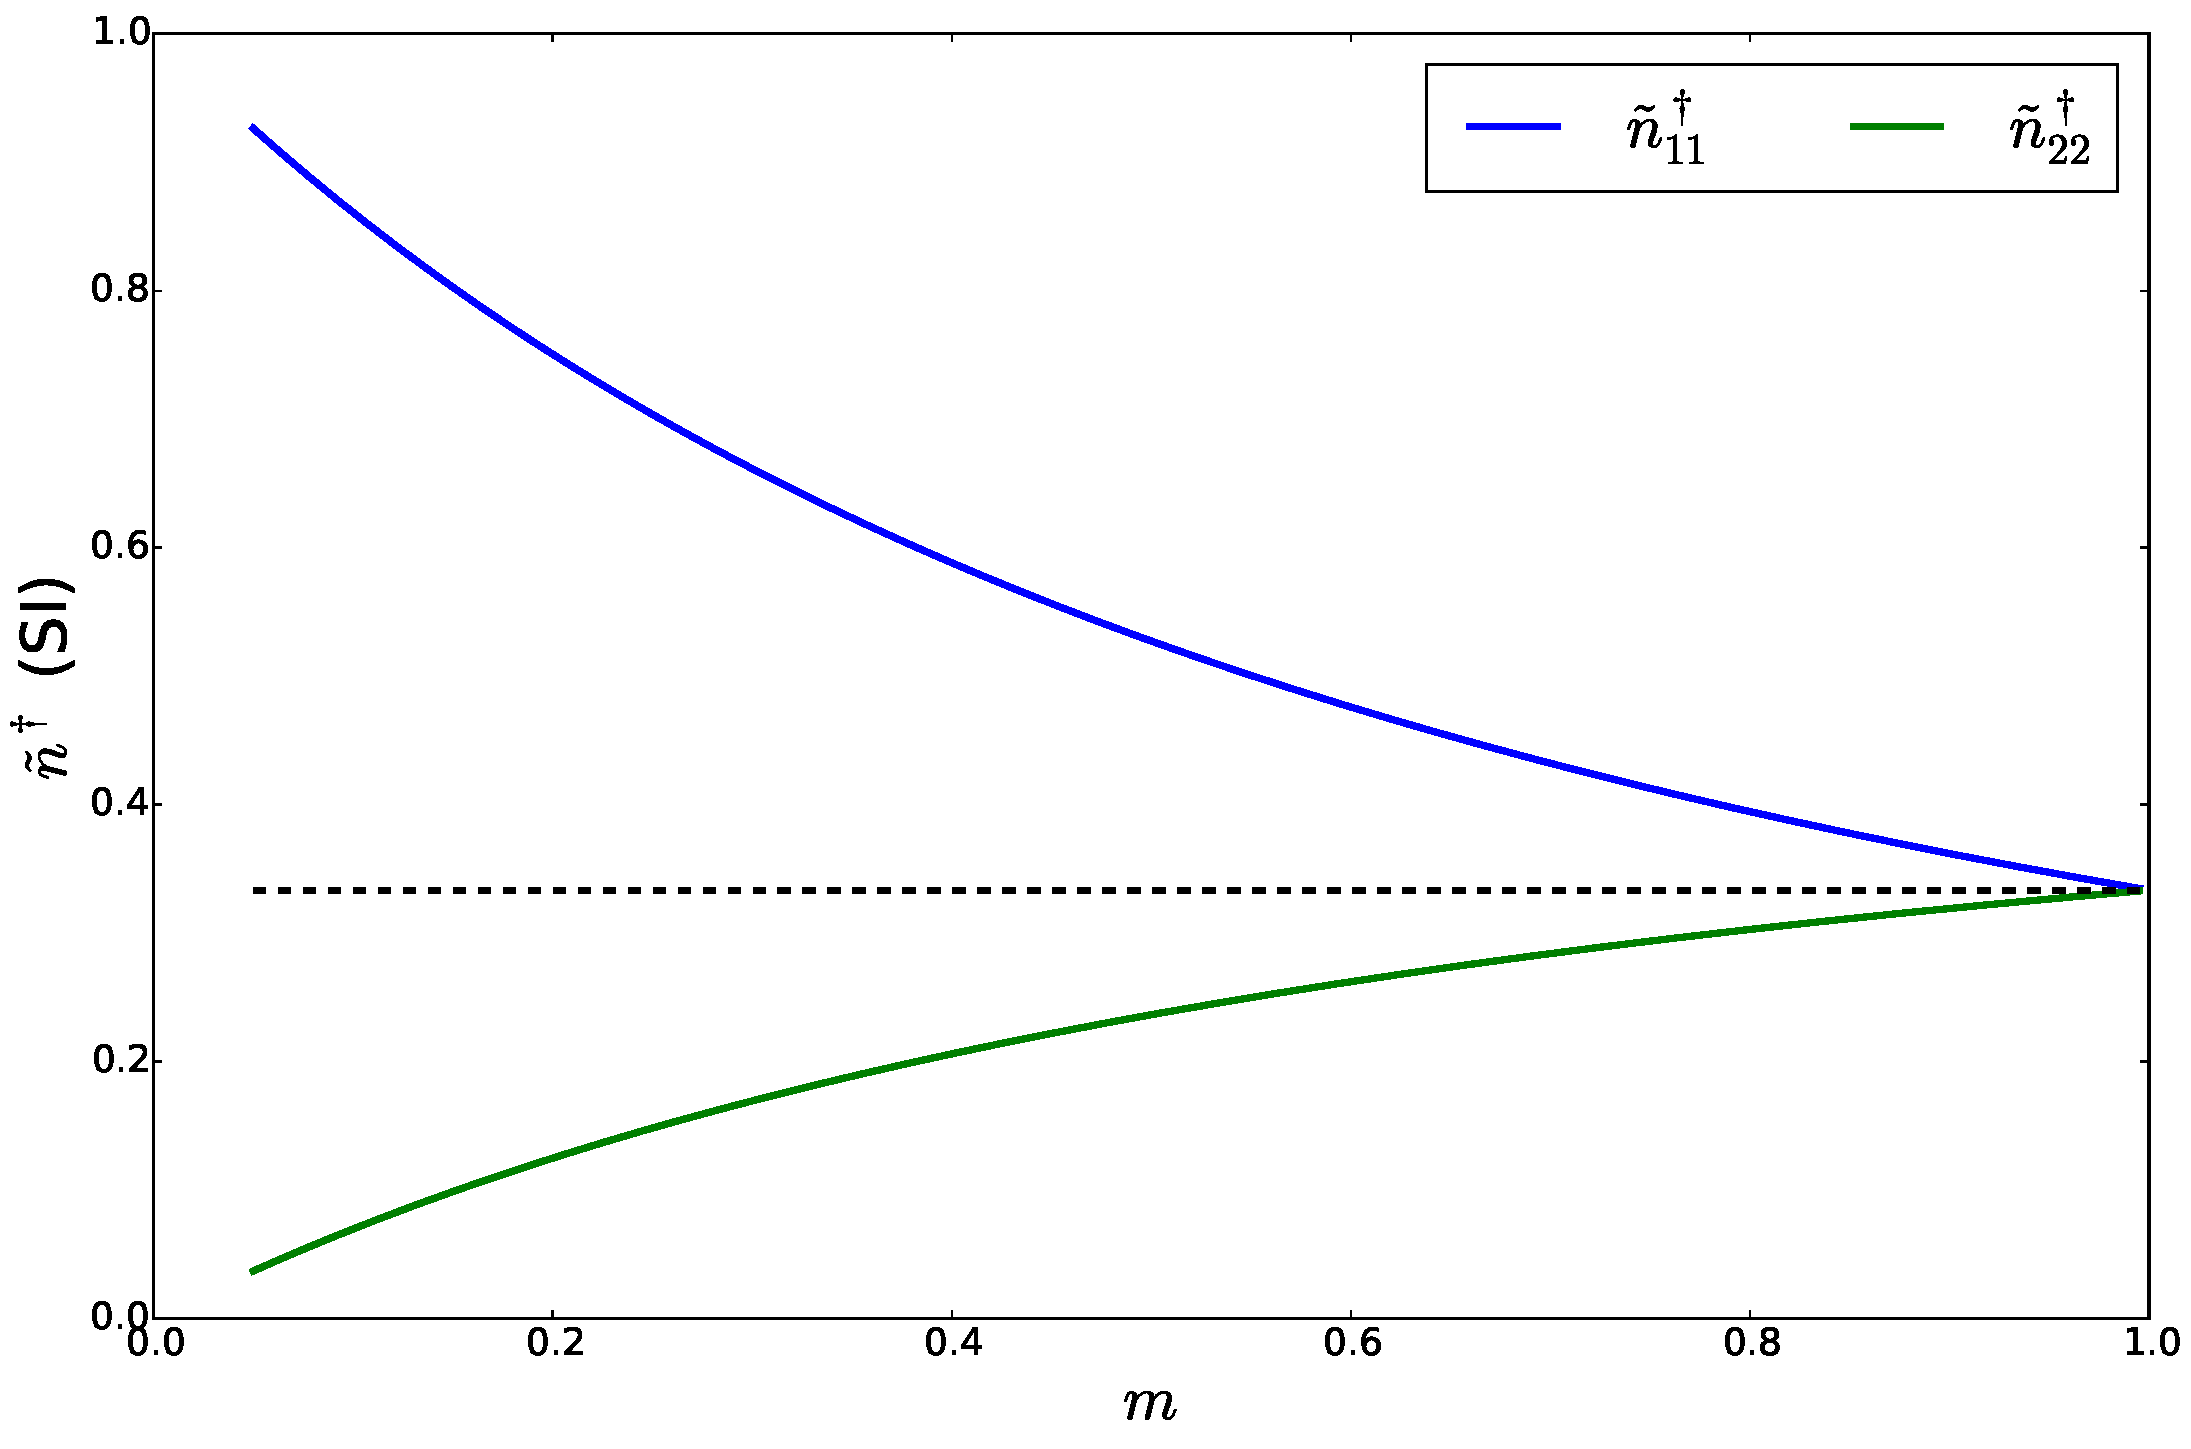
\includegraphics[width=15cm,height=10cm]{figures/test_n_oblate}
	\caption[Teste dos fatores de desmagnetização para um elipsoide oblato.]{Teste dos fatores de desmagnetização:
		$\tilde{n}^{\dagger}_{11}$ e $\tilde{n}^{\dagger}_{22}$
		para um elipsoide oblato originalmente com semi-eixos 1000 e 50 metros, com um fator $u (a/b)$ crescente,
		mantendo o semi-eixo maior constante (neste caso o $b$), e tornando o semi-eixo menor maior, até o ponto de
		quase se igualarem.}
	\label{fig:n_oblato}
\end{figure}

Através destes gráficos é possível observar como os fatores de desmagnetização possuem valor menor, quanto maior o semi-eixo do elipsoide. De fato há uma relação: $\tilde{n}^{\dagger}_{11}$ está relacionado com o semi-eixo maior, $\tilde{n}^{\dagger}_{22}$ com o semi-eixo intermediário e $\tilde{n}^{\dagger}_{33}$ com o semi-eixo menor. Fisicamente, isto significa que há a tendência, do elipsoide se desmagnetizar com maior intensidade na direção dos seus semi-eixos menores.

\section{Comparações entre os modelos elipsoidais}

Testamos a implementação computacional comparando com resultados conhecidos. Na Figura \ref{fig:triaxial_sphere} comparamos um elipsoide triaxial com seus três semi-eixos muito próximos um do outro (simulando uma esfera), conforme Tabela 4.5, e comparamos com a implementação da esfera do software \textit{Fatiando a Terra}.
\newpage

\begin{table}[h!]
	\begin{center}
		\begin{tabular}{lc}
			
			&  \\
			& \\
			& \\
			& \\
			& \\
			& \\
			& \\
			& \\
			& \\
			& \\
			& \\
			& \\
			& \\
		\end{tabular}
	\end{center}
\end{table}

\begin{table}[h!]
	\begin{center}
		\begin{tabular}{|l|c|c|}
			\hline
			\textbf{Parâmetro}  & \textbf{Valor}  & \textbf{Unidade}\\
			\hline 
			a, b, c   & 500.0001, 500.0, 499.9999   & m\\
			\hline
			Azimute   & $0$ & º\\
			\hline
			$\delta$    & $0$ & º\\
			\hline
			$\gamma$   & $0$  & º\\
			\hline
			xc   & 0  & m\\
			\hline          
			yc   & 0  & m\\
			\hline                
			zc   & 1000  & m\\
			\hline
			$J_{NRM}$*  & 100, $25^o$, $40^o$  & A/m\\
			\hline
			F*    & 1, $50^o$, $20^o$ & nT\\
			\hline
			k1, k2, k3   & 0.1, 0.1, 0.1 & SI \\
			\hline
			Orientações k**   & $0$, $90$, $90$  & º\\
			\hline
		\end{tabular}
		\caption{Parâmetros do elipsoide triaxial modelado. *Valores de intensidade, inclinação e declinação respectivamente. **Ângulo de \textit{strike} , \textit{dip}  e \textit{rake} , respectivamente, para calcular os vetores unitários $\mathbf{u}_{1}$, $\mathbf{u}_{2}$, $\mathbf{u}_{3}$ por meio das Eqs. \ref{eq:v1_triaxial_prolate}, \ref{eq:v2_triaxial_prolate} e \ref{eq:v3_triaxial_prolate}.}
	\end{center}
	\label{tab:triaxial_sphere}
\end{table}

\begin{table}[h!]
	\begin{center}
		\begin{tabular}{lc}
			
			&  \\
			& \\
			& \\
			& \\
			& \\
			& \\
			& \\
			& \\
			& \\
			& \\
			& \\
			& \\
				
		\end{tabular}
	\end{center}
\end{table}

\begin{figure}[hbt!]
	\centering 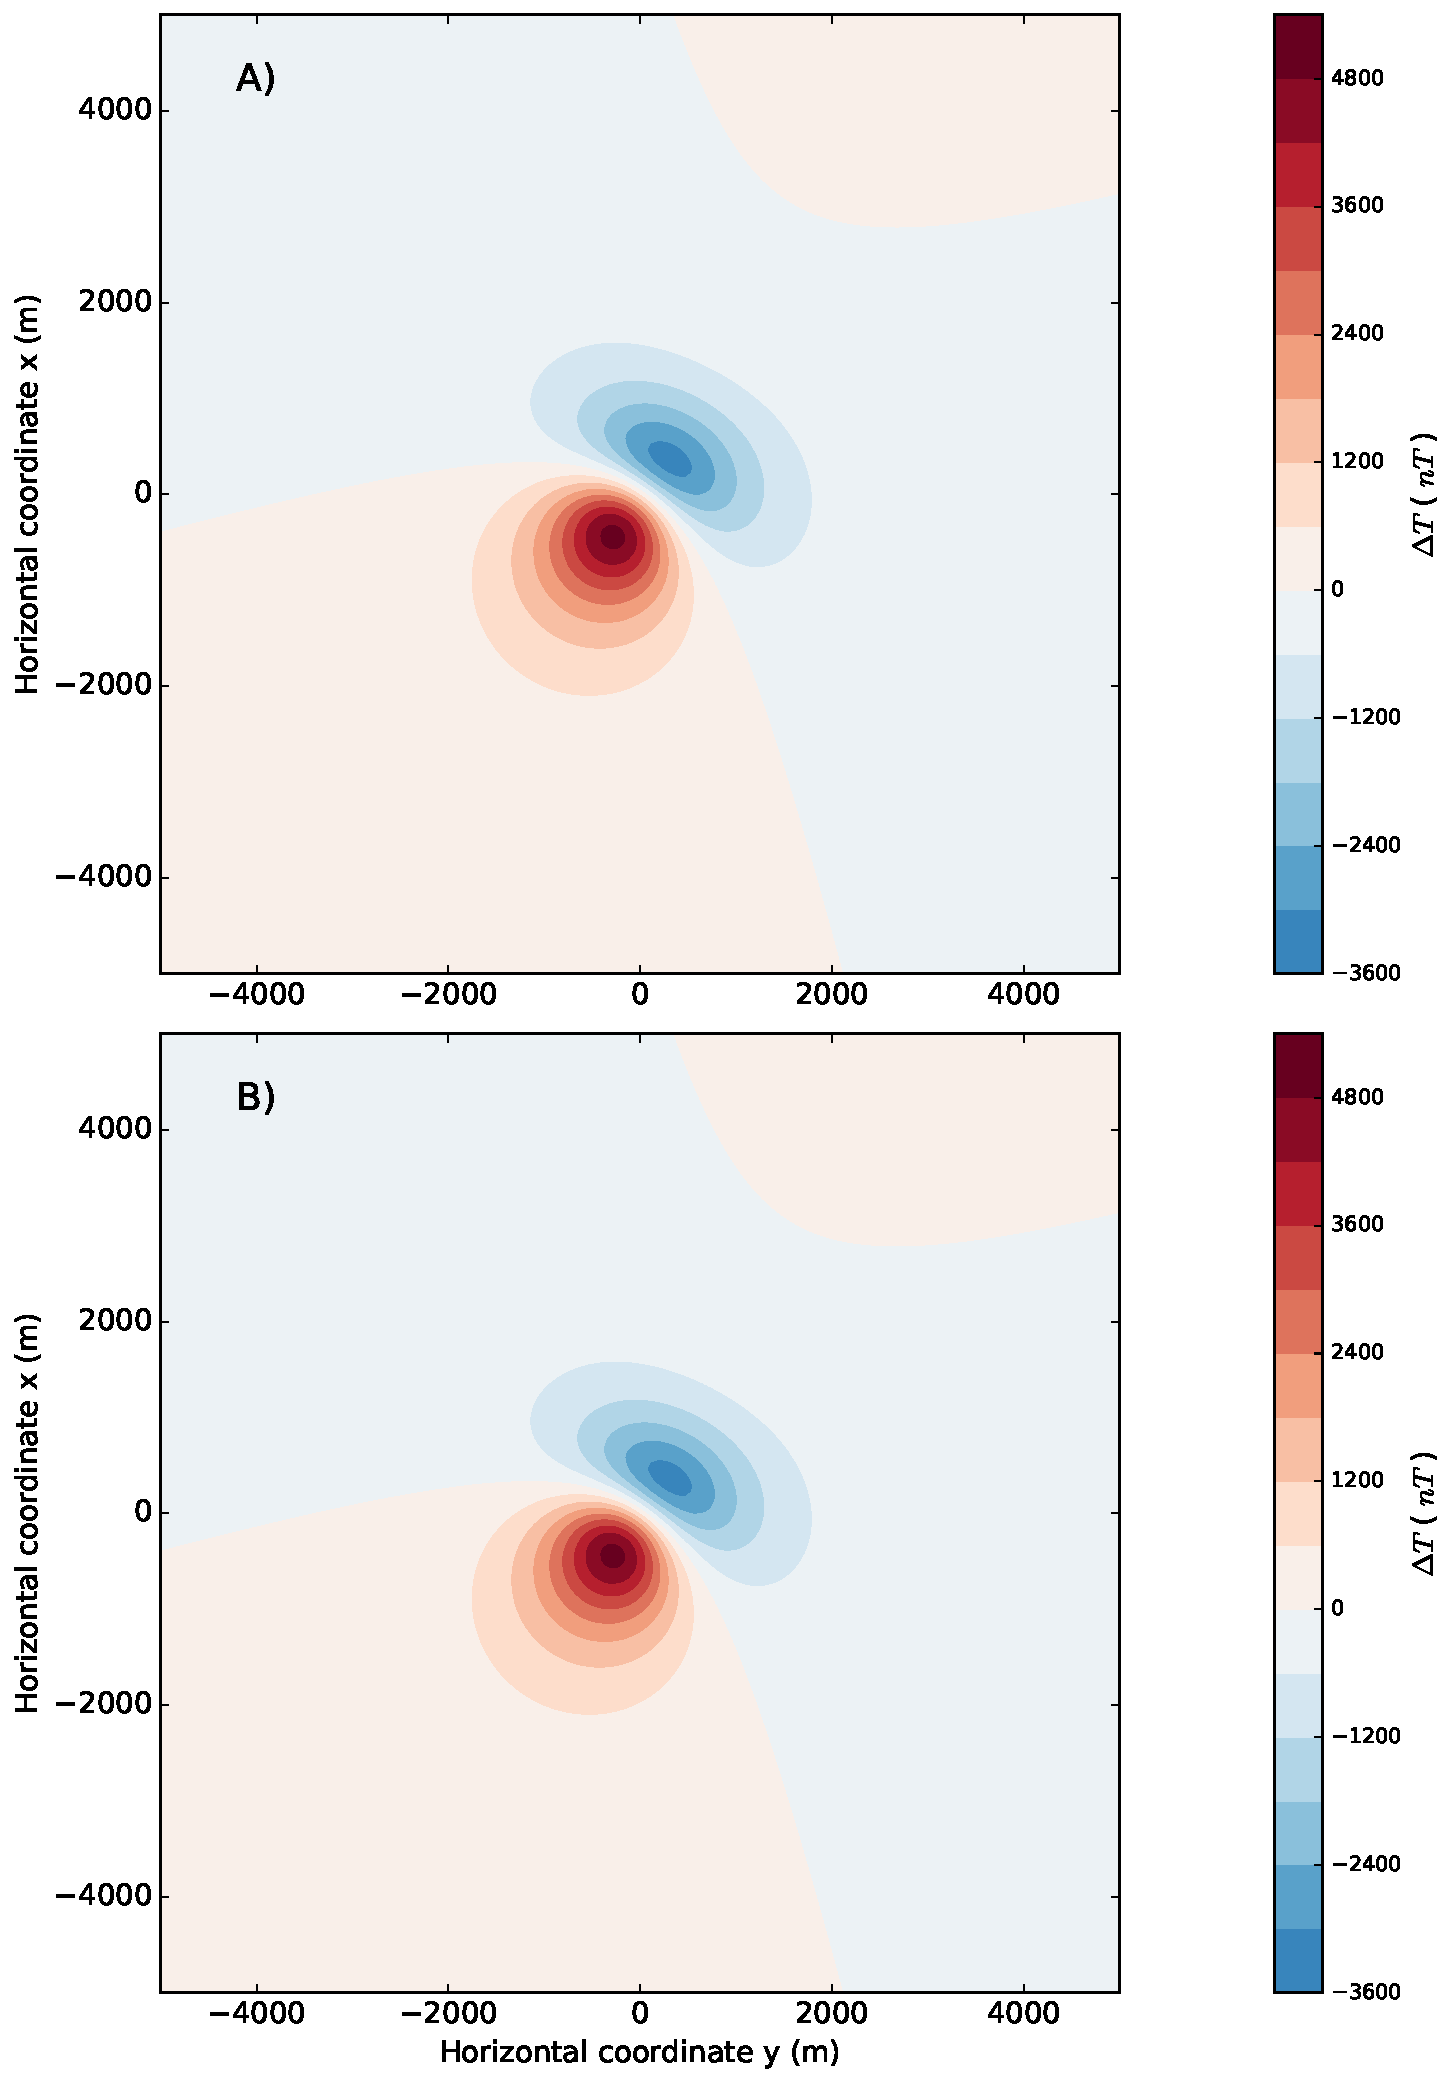
\includegraphics[width=14.5 cm,height=22 cm]{figures/ellipsoid_triaxial_sphere}
	\caption[Comparação da anomalia de campo total aproximada entre um elipsoide triaxial com três semi-eixos muito próximos, simulando uma esfera, 
	e uma esfera.]{Comparação da anomalia de campo total aproximada entre um elipsoide triaxial com três semi-eixos muito próximos, simulando uma esfera, e uma esfera implementada pelo software \textit{Fatiando a Terra}.}
	\label{fig:triaxial_sphere}
\end{figure}

Os resultados da comparação foram muito próximos. Confirmado a implementação do elipsoide triaxial, o usamos para comparar com a implementação do elipsoide prolato de parâmetros conforme tabelas 4.6 e 4.7. O resultado está na Figura \ref{fig:triaxial_prolate}.

\begin{table}[h!]
	\begin{center}
		\begin{tabular}{|l|c|c|}
			\hline
			\textbf{Parâmetro}  & \textbf{Valor}  & \textbf{Unidade} \\
			\hline 
			a, b, c  & 500, 100, 99.99 & m\\
			\hline
			Azimute   & $90$ & º\\
			\hline
			$\delta$    & $45$ & º\\
			\hline
			$\gamma$   & $0$  & º\\
			\hline
			xc   & 0 & m \\
			\hline          
			yc   & 0  & m\\
			\hline                
			zc   & 1000  & m\\
			\hline
			$J_{NRM}$*  & 100, $90^o$, $0^o$  & nT\\
			\hline
			F*    & 60000, $50^o$, $20^o$ & A/m\\
			\hline
			k1, k2, k3   & 0.2, 0.1, 0.05  & SI\\
			\hline
			Orientações k**   & $0$, $90$, $90$  & º\\
			\hline
		\end{tabular}
		\caption{Parâmetros do elipsoide triaxial modelado. *Valores de intensidade, inclinação e declinação respectivamente. **Ângulo de \textit{strike} , \textit{dip}  e \textit{rake} , respectivamente, para calcular os vetores unitários $\mathbf{u}_{1}$, $\mathbf{u}_{2}$, $\mathbf{u}_{3}$ por meio das Eqs. \ref{eq:v1_triaxial_prolate}, \ref{eq:v2_triaxial_prolate} e \ref{eq:v3_triaxial_prolate}.}
	\end{center}
	\label{tab:triaxial_prolate1}
\end{table}

\vspace{2cm}

\begin{table}[h!]
	\begin{center}
		\begin{tabular}{|l|c|c|}
			\hline
			\textbf{Parâmetro}  & \textbf{Valor}  & \textbf{Unidade}\\
			\hline 
			a, b  & 500, 100 & m\\
			\hline
			Azimute   & $90$ & m\\
			\hline
			$\delta$    & $45$ & º\\
			\hline
			$\gamma$   & $0$  & º\\
			\hline
			xc   & 0  & m\\
			\hline          
			yc   & 0  & m\\
			\hline                
			zc   & 1000  & m\\
			\hline
			$J_{NRM}$*  & 100, $90^o$, $0^o$  & A/m\\
			\hline
			F*    & 60000, $50^o$, $20^o$ & nT\\
			\hline
			k1, k2, k3   & 0.2, 0.1, 0.05  & SI\\
			\hline
			Orientações k**   & $0$, $90$, $90$  & º\\
			\hline
		\end{tabular}
		\caption{Parâmetros do elipsoide triaxial modelado. *Valores de intensidade, inclinação e declinação respectivamente. **Ângulo de \textit{strike} , \textit{dip}  e \textit{rake} , respectivamente, para calcular os vetores unitários $\mathbf{u}_{1}$, $\mathbf{u}_{2}$, $\mathbf{u}_{3}$ por meio das Eqs. \ref{eq:v1_triaxial_prolate}, \ref{eq:v2_triaxial_prolate} e \ref{eq:v3_triaxial_prolate}.}
	\end{center}
	\label{tab:triaxial_prolate2}
\end{table}

\begin{figure}[hbt!]
	\centering \includegraphics[width=14.5 cm,height=22 cm]{figures/ellipsoid_triaxial_prolate}
	\caption[Comparação da anomalia de campo total aproximada entre um elipsoide triaxial com um dos semi-eixos mais alongado que o 
	restante e um elipsoide prolato.]{Comparação da anomalia de campo total aproximada entre um elipsoide triaxial com um dos semi-eixos mais alongado que o restante e um elipsoide prolato.}
	\label{fig:triaxial_prolate}
\end{figure}

Também usamos a implementação do elipsoide triaxial, para comparar com a implementação do elipsoide oblato de parâmetros conforme tabelas 4.8 e 4.9. O resultado está na Figura \ref{fig:triaxial_oblate}.

\begin{table}[h!]
	\begin{center}
		\begin{tabular}{|l|c|c|}
			\hline
			\textbf{Parâmetro}  & \textbf{Valor} & \textbf{Unidade} \\
			\hline 
			a, b, c   & 500, 499.99, 499.98 & m\\
			\hline
			Azimute   & $0$ & m\\
			\hline
			$\delta$    & $0$ & º\\
			\hline
			$\gamma$   & $90$  & º\\
			\hline
			xc   & 0  & m\\
			\hline          
			yc   & 0  & m\\
			\hline                
			zc   & 1000 & m \\
			\hline
			$J_{NRM}$*  & 100, $90^o$, $0^o$ & A/m \\
			\hline
			F*    & 60000, $50^o$, $20^o$ & nT \\
			\hline
			k1, k2, k3   & 0.1, 0.1, 0.1 & SI \\
			\hline
			Orientações k**   & $0$, $90$, $90$ & º \\
			\hline
		\end{tabular}
		\caption{Parâmetros do elipsoide triaxial modelado. *Valores de intensidade, inclinação e declinação respectivamente. **Ângulo de \textit{strike} , \textit{dip}  e \textit{rake} , respectivamente, para calcular os vetores unitários $\mathbf{u}_{1}$, $\mathbf{u}_{2}$, $\mathbf{u}_{3}$ por meio das Eqs. \ref{eq:v1_triaxial_prolate}, \ref{eq:v2_triaxial_prolate} e \ref{eq:v3_triaxial_prolate}.}
	\end{center}
	\label{tab:triaxial_oblate1}
\end{table}

\vspace{2cm}

\begin{table}[h!]
	\begin{center}
		\begin{tabular}{|l|c|c|}
			\hline
			\textbf{Parâmetro}  & \textbf{Valor} & \textbf{Unidade} \\
			\hline 
			a, b   & 499.99, 500 & m\\
			\hline
			Azimute   & $0$ & º\\
			\hline
			$\delta$    & $0$ & º\\
			\hline
			$\gamma$   & $0$  & º\\
			\hline
			xc   & 0  & m\\
			\hline          
			yc   & 0  & m\\
			\hline                
			zc   & 1000  & m\\
			\hline
			$J_{NRM}$*  & 100, $90^o$, $0^o$  & A/m\\
			\hline
			F*    & 60000, $50^o$, $20^o$ & nT \\
			\hline
			k1, k2, k3   & 0.1, 0.1, 0.1 & SI \\
			\hline
			Orientações k**   & $0$, $90$, $90$ & º \\
			\hline
		\end{tabular}
		\caption{Parâmetros do elipsoide triaxial modelado. *Valores de intensidade, inclinação e declinação respectivamente. **Ângulo de \textit{strike} , \textit{dip}  e \textit{rake} , respectivamente, para calcular os vetores unitários $\mathbf{u}_{1}$, $\mathbf{u}_{2}$, $\mathbf{u}_{3}$ por meio das Eqs. \ref{eq:v1_triaxial_prolate}, \ref{eq:v2_triaxial_prolate} e \ref{eq:v3_triaxial_prolate}.}
	\end{center}
	\label{tab:triaxial_oblate2}
\end{table}

\begin{figure}[hbt!]
	\centering \includegraphics[width=14.5 cm,height=22 cm]{figures/ellipsoid_triaxial_oblate}
	\caption[Comparação da anomalia de campo total aproximada entre um elipsoide triaxial com três semi-eixos muito próximos 
	e um elipsoide oblato.]{Comparação da anomalia de campo total aproximada entre um elipsoide triaxial com três semi-eixos muito próximos e um elipsoide oblato também com seus dois semi-eixos muito próximos.}
	\label{fig:triaxial_oblate}
\end{figure}

\section{Susceptibilidade}

Em corpos de alta susceptibilidade, a desmagnetização é um fator muito importante, pois isso pode acarretar em erros de interpretação das anomalias em dados magnéticos. Na Figura \ref{fig:test_k_triaxial}, mostramos com um aumento gradual da susceptibilidade (neste caso isotrópica), a diferença na inclinação e declinação que o vetor de magnetização resultante sofre. É conhecido na literatura que o valor de susceptibilidade de 0.1 SI é o ponto onde a desmagnetização não deve ser desconsiderada na modelagem, o que de fato observa-se neste gráfico.

\begin{figure}[hbt!]
	\centering 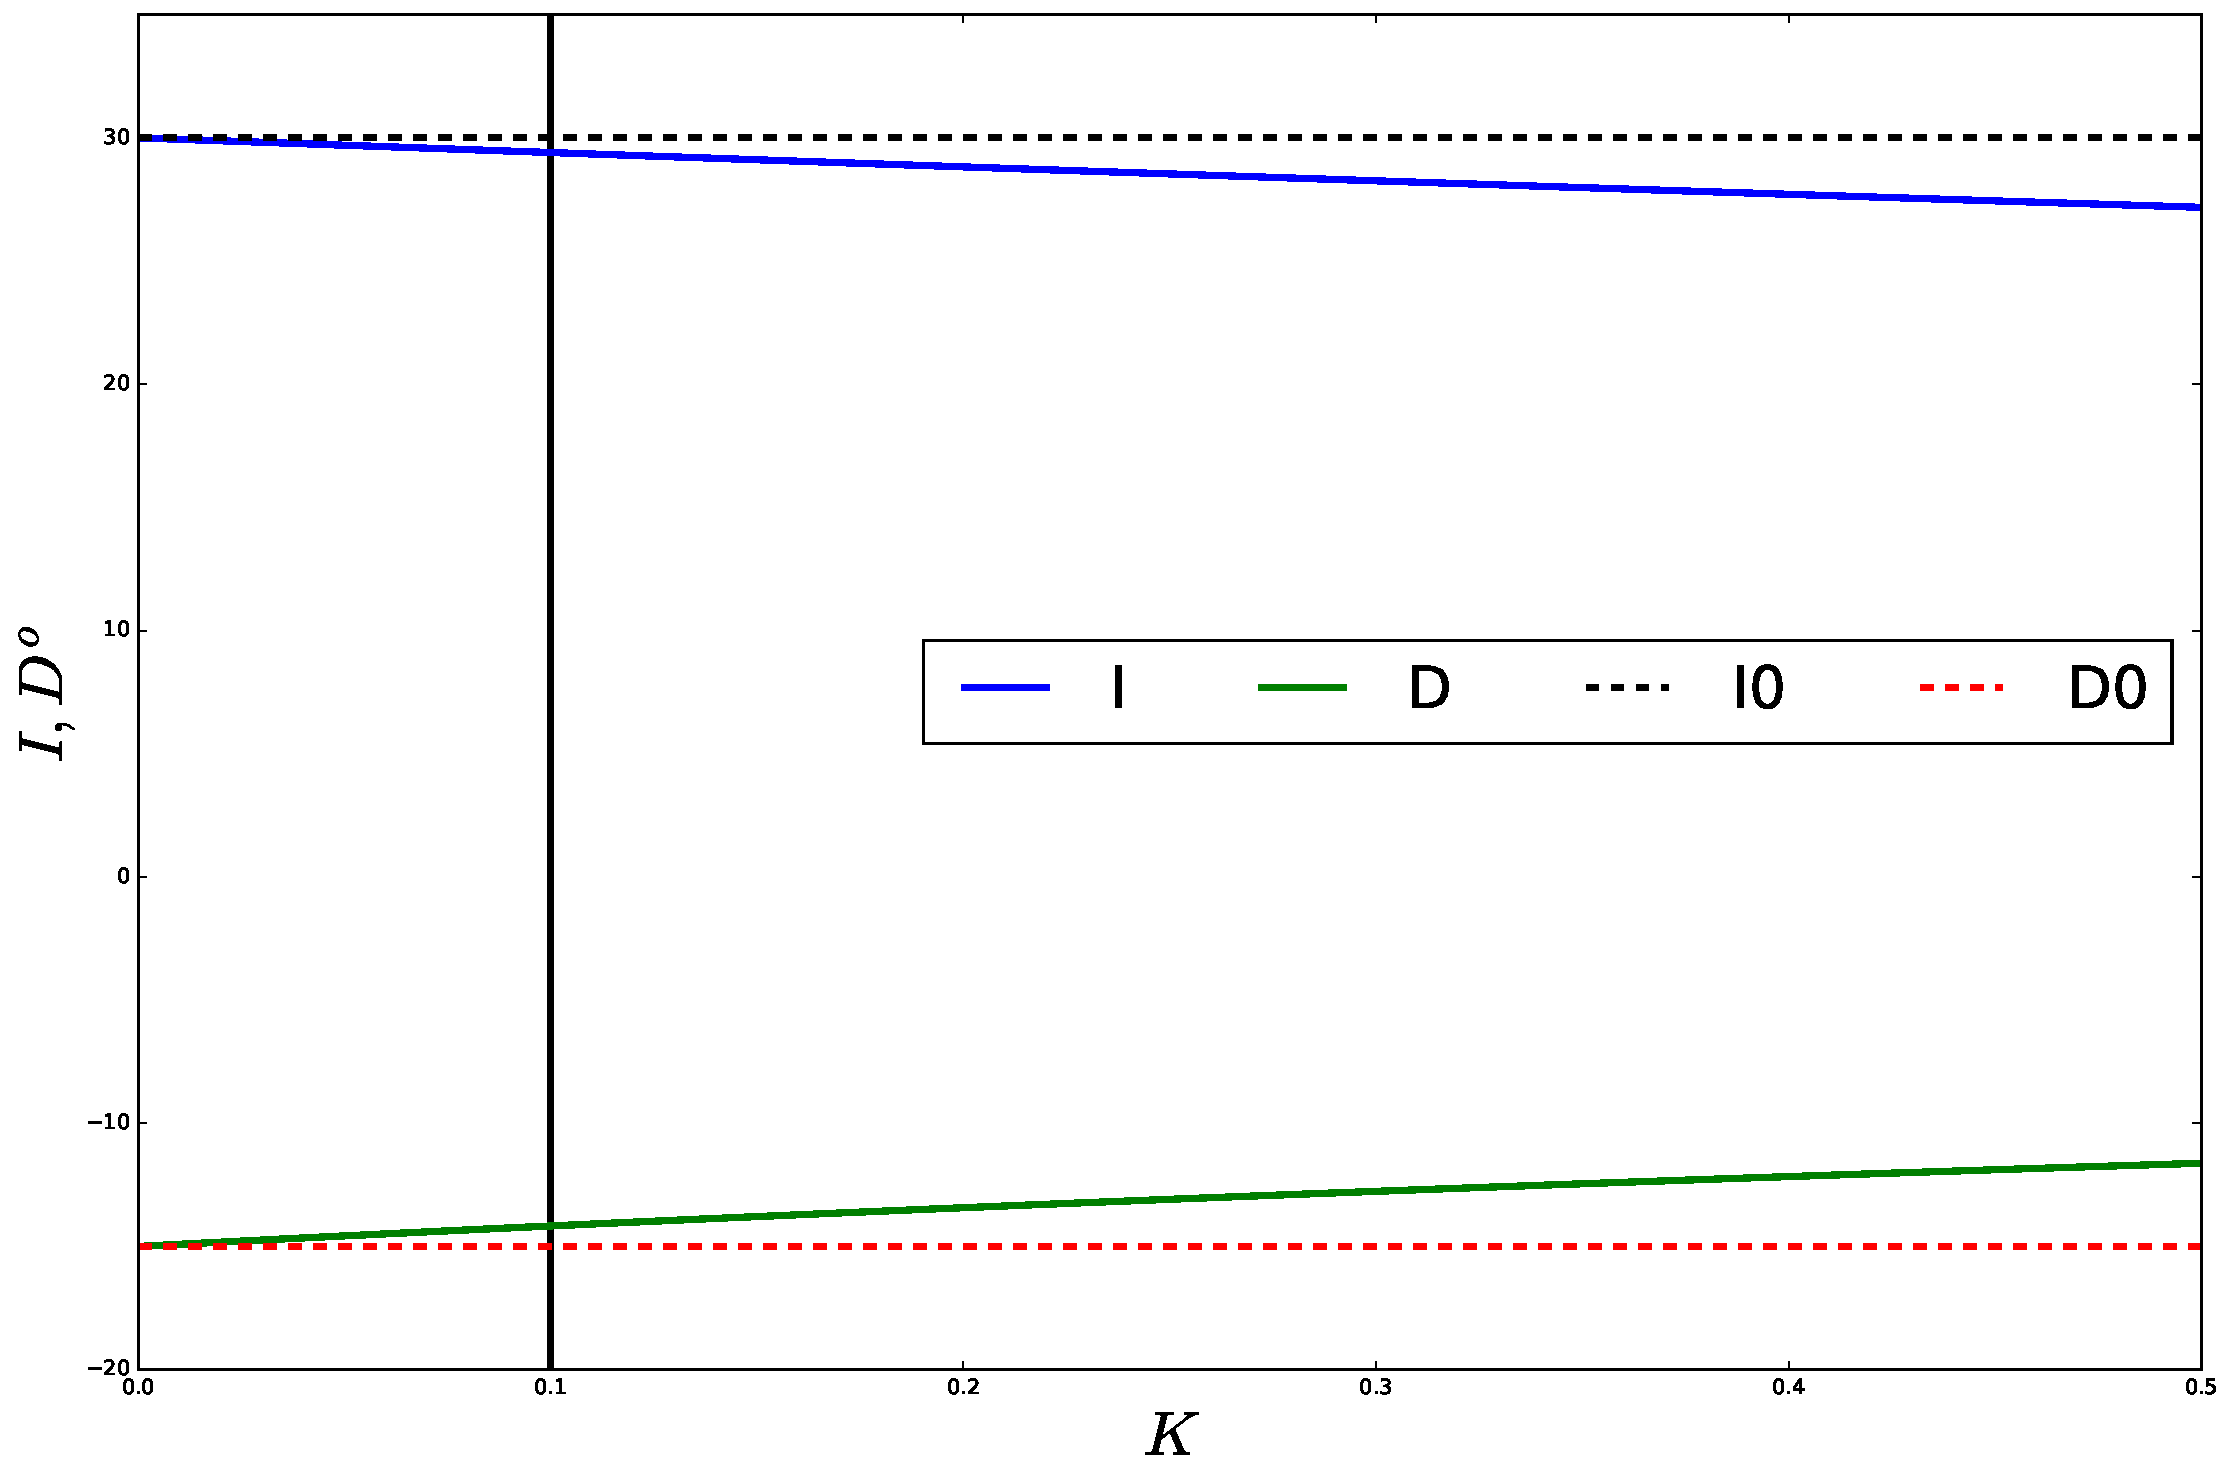
\includegraphics[width=15 cm,height=10 cm]{figures/test_k_triaxial}
	\caption[Teste do efeito da susceptibilidade na desmagnetização de um elipsoide imerso em um campo externo constante de inclinação 
	$30^{o}$ e declinação $-15^{o}$.]{Teste do efeito da susceptibilidade na desmagnetização de um elipsoide imerso em um campo externo constante de inclinação	$30^{o}$ e declinação $-15^{o}$, sem magnetização remanente, que recebe gradativamente, de forma isotrópica,
		uma susceptibilidade crescente. Em destaque uma linha demarcatória em $K=0.1$ SI, onde a literatura reconhece como um valor limite 
		para desconsiderar os efeitos da desmagnetização.}
	\label{fig:test_k_triaxial}
\end{figure}

\begin{table}[h!]
	\begin{center}
		\begin{tabular}{lc}
			
			&  \\
			& \\
			& \\
			& \\
			& \\
			
		\end{tabular}
	\end{center}
\end{table}

\section{Anisotropia de forma}

Conforme dito na seção 4.2 existe uma relação entre os elementos do tensor de depolarização e os semi-eixos. Na Figura \ref{fig:ellipsoid_shape_iso10} mostramos como o aumento do semi-eixo maior afeta o vetor de magnetização resultante. A princípio, os três semi-eixos estão muito próximos, simulando uma esfera. Quando postos sob um campo externo, o vetor de magnetização resultante se direciona para a direção deste campo. Porém a medida que aumenta-se o semi-eixo maior, ocorre a depolarização dos demais e o vetor de magnetização resultante tende a se alinhar na direção do semi-eixo maior (neste caso o elipsoide triaxial possui um azimute de 10$º$).

\vspace{2cm}

\begin{table}[h!]
	\begin{center}
		\begin{tabular}{|l|c|c|}
			\hline
			\textbf{Parâmetro}  & \textbf{Valor}  & \textbf{Unidade }\\
			\hline 
			a, b, c  & 50.1-1000, 50, 49.9 & m\\
			\hline
			Azimute   & $10$ & º \\
			\hline
			$\delta$    & $0$ & º\\
			\hline
			$\gamma$   & $0$  & º\\
			\hline
			xc   & 0  & m\\
			\hline          
			yc   & 0  & m\\
			\hline                
			zc   & 1000  & m\\
			\hline
			$J_{NRM}$*  & 100, $0^o$, $0^o$ & A/m \\
			\hline
			F*    & 60000, $90^o$, $20^o$ & nT\\
			\hline
			k1, k2, k3   & 50, 50, 50  & SI\\
			\hline
			Orientações k**   & $0$, $90$, $90$  & º\\
			\hline
		\end{tabular}
		\caption{Parâmetros do elipsoide triaxial modelado. *Valores de intensidade, inclinação e declinação respectivamente. **Ângulo de \textit{strike} , \textit{dip}  e \textit{rake} , respectivamente, para calcular os vetores unitários $\mathbf{u}_{1}$, $\mathbf{u}_{2}$, $\mathbf{u}_{3}$ por meio das Eqs. \ref{eq:v1_triaxial_prolate}, \ref{eq:v2_triaxial_prolate} e \ref{eq:v3_triaxial_prolate}.}
	\end{center}
	\label{tab:ellipsoid_shape_iso10}
\end{table}

\begin{table}[h!]
	\begin{center}
		\begin{tabular}{lc}
			
			&  \\
			& \\
			& \\
			&  \\
			& \\
			& \\
			& \\
			& \\
			& \\
			& \\

			
		\end{tabular}
	\end{center}
\end{table}

\begin{figure}[hbt!]
	\centering 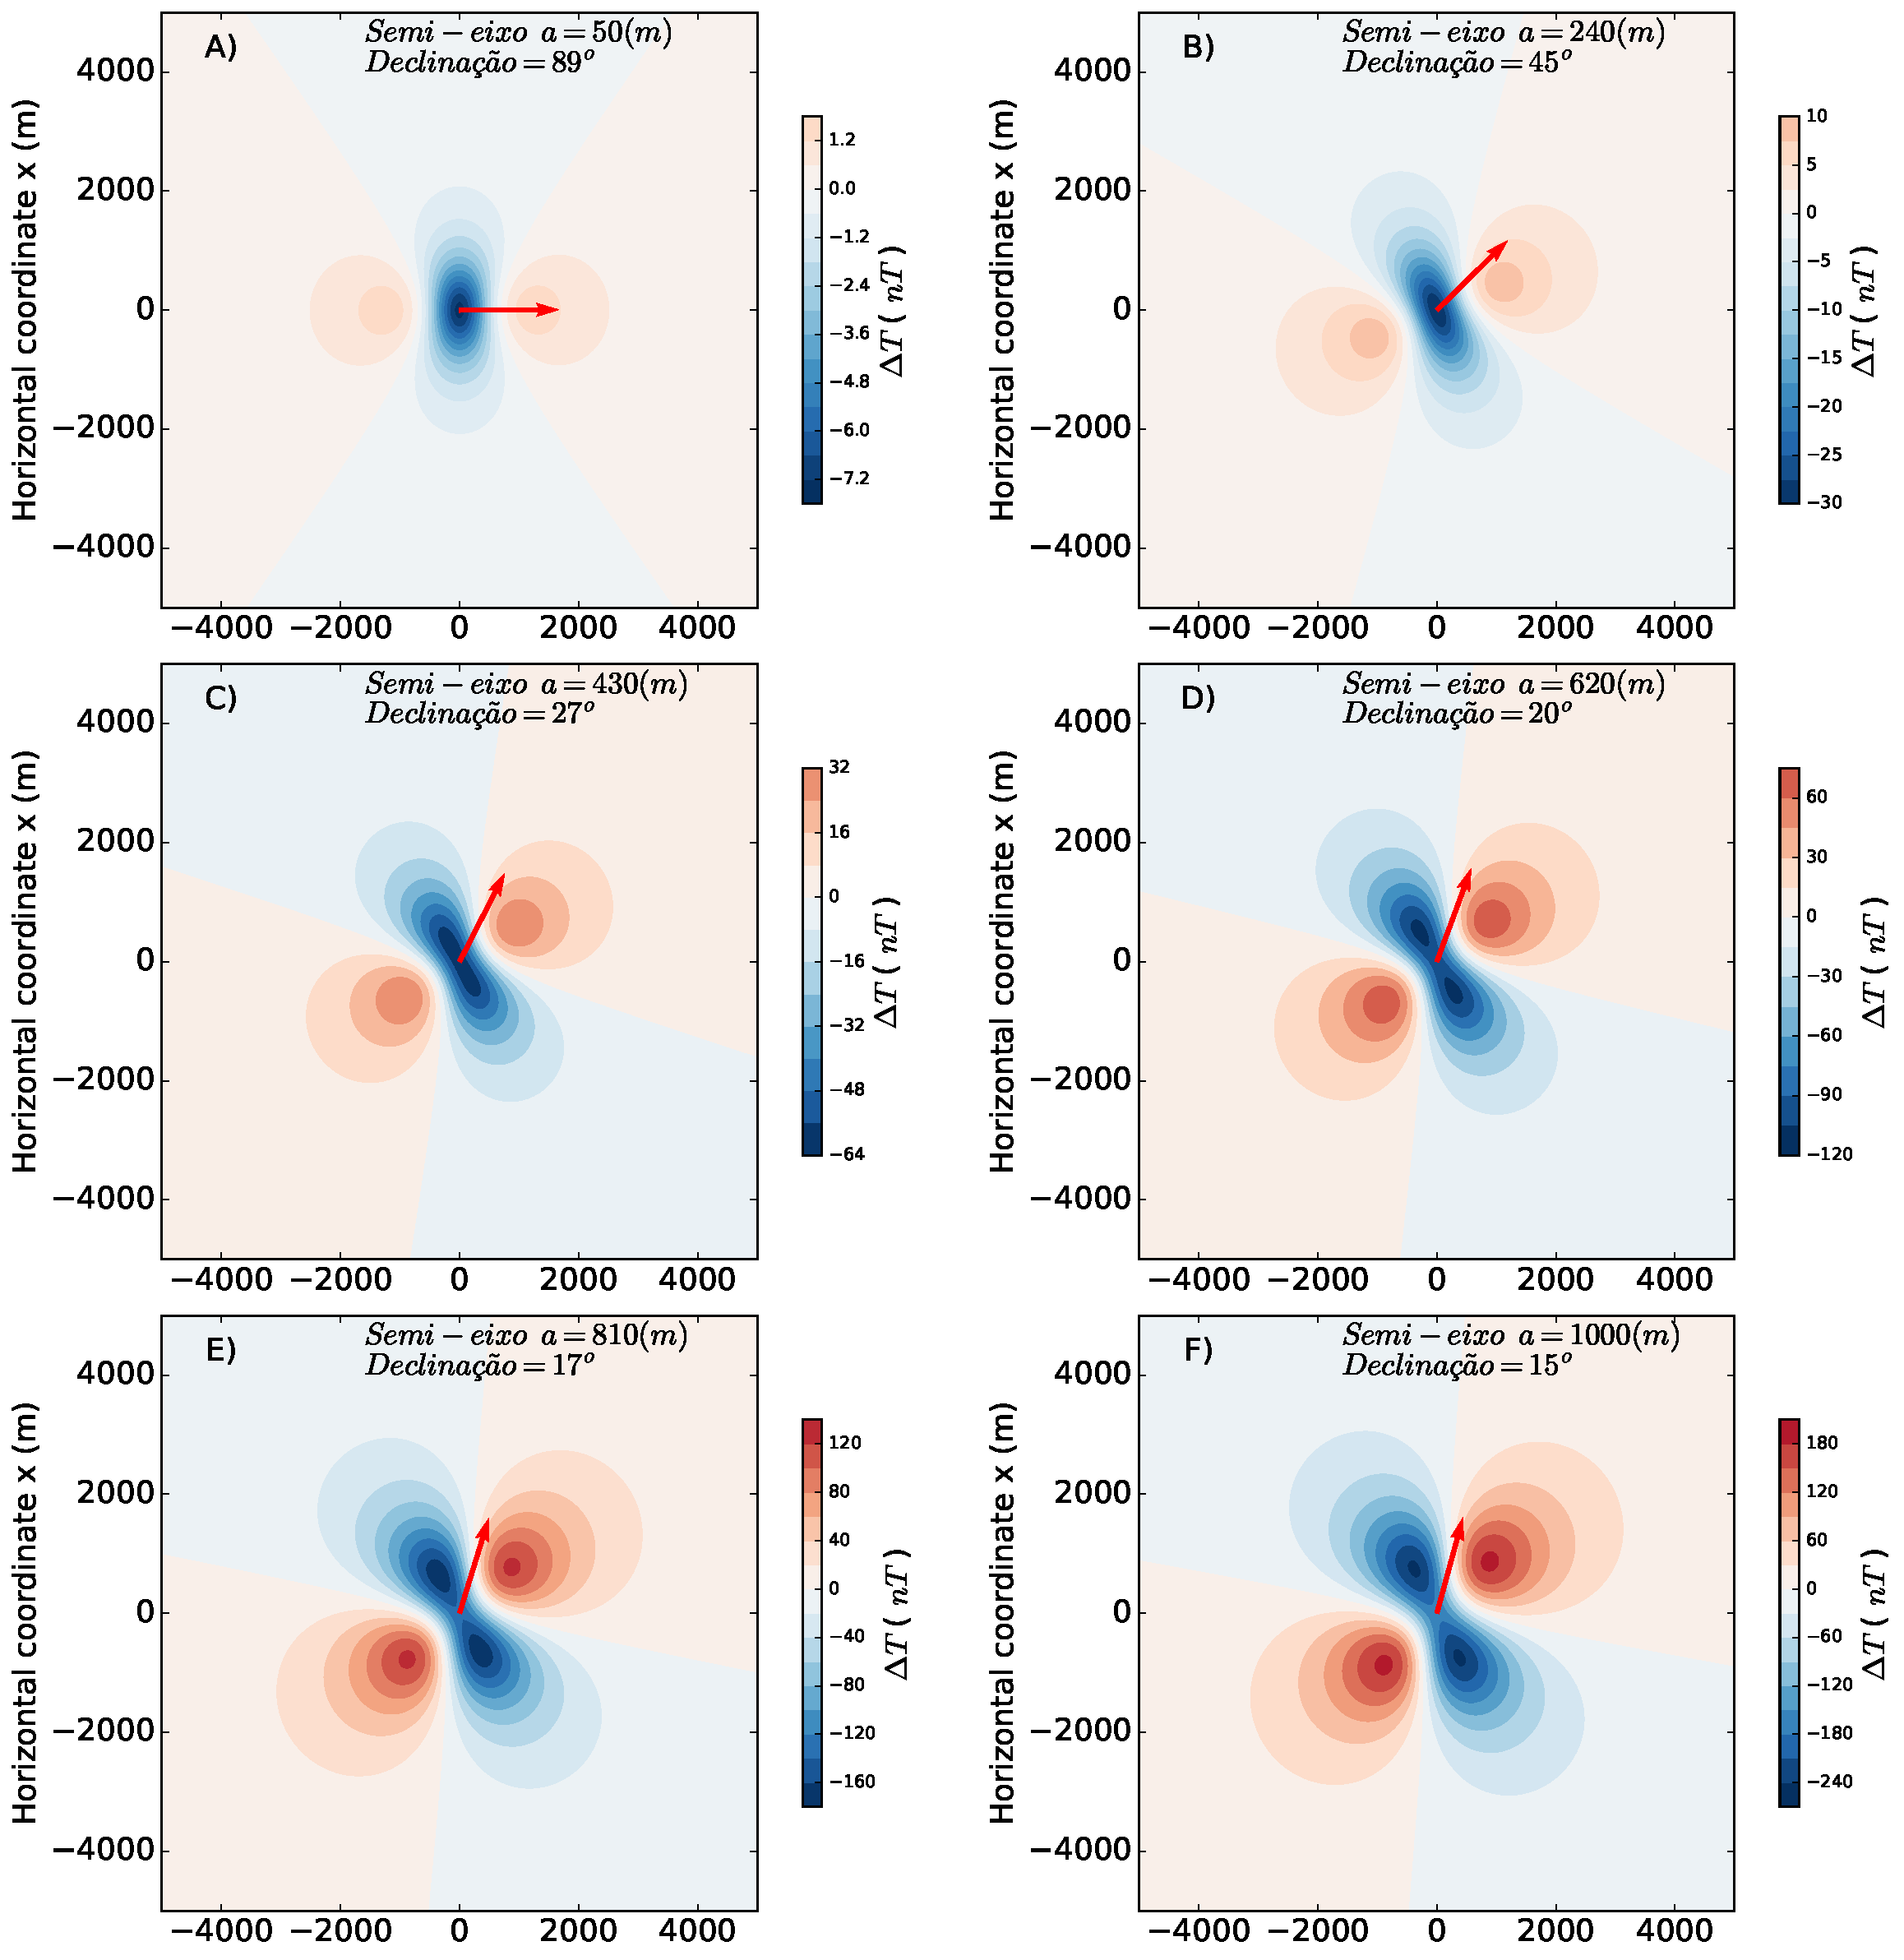
\includegraphics[width=16 cm,height=16 cm]{figures/ellipsoid_shape_iso}
	\caption[Simulação, da mudança do vetor de magnetização resultante, de um elipsoide triaxial com o aumento do semi-eixo maior.]{Simulação, da mudança do vetor de magnetização resultante, de um elipsoide triaxial com o aumento do semi-eixo maior. O elipsoide está imerso em um campo externo constante de declinação $90^o$, possui susceptibilidade isotrópica e constante e está direcionado com um azimute de $10^o$. Ao longo da sequência das figuras, seu semi-eixo maior aumenta de proporção em relação aos demais (variando entre 50 e 3000 m.). Nota-se a tendência do vetor de magnetização resultante (seta em vermelho) em se alinhar com o semi-eixo maior.}
	\label{fig:ellipsoid_shape_iso10}
\end{figure}

\begin{table}[h!]
	\begin{center}
		\begin{tabular}{lc}
			
			& \\
			& \\
			& \\
			& \\
			& \\
			
		\end{tabular}
	\end{center}
\end{table}

Para efeito de comparação realizamos o mesmo teste, porém com um azimute de 80$º$ para o elipsoide. A variação é bem menor, mas também se confirma a tendência do alinhamento do vetor de magnetização resultante para a direção do semi-eixo maior.

\vspace{2cm}

\begin{table}[h!]
	\begin{center}
		\begin{tabular}{|l|c|c|}
			\hline
			\textbf{Parâmetro}  & \textbf{Valor}  & \textbf{Unidade} \\
			\hline 
			a, b, c & 50.1-1000, 50, 49.9 & m\\
			\hline
			Azimute   & $80$ & º\\
			\hline
			$\delta$    & $0$ & º\\
			\hline
			$\gamma$   & $0$  & º\\
			\hline
			xc   & 0  & m\\
			\hline          
			yc   & 0  & m\\
			\hline                
			zc   & 1000  & m\\
			\hline
			$J_{NRM}$*  & 100, $0^o$, $0^o$  & A/m\\
			\hline
			F*    & 60000, $50^o$, $20^o$ & nT\\
			\hline
			k1, k2, k3   & 50, 50, 50  & SI\\
			\hline
			Orientações k**   & $0$, $90$, $90$  & º\\
			\hline
		\end{tabular}
		\caption{Parâmetros do elipsoide triaxial modelado. *Valores de intensidade, inclinação e declinação respectivamente. **Ângulo de \textit{strike} , \textit{dip}  e \textit{rake} , respectivamente, para calcular os vetores unitários $\mathbf{u}_{1}$, $\mathbf{u}_{2}$, $\mathbf{u}_{3}$ por meio das Eqs. \ref{eq:v1_triaxial_prolate}, \ref{eq:v2_triaxial_prolate} e \ref{eq:v3_triaxial_prolate}.}
	\end{center}
	\label{tab:ellipsoid_shape_iso80}
\end{table}

\begin{figure}[hbt!]
	\centering 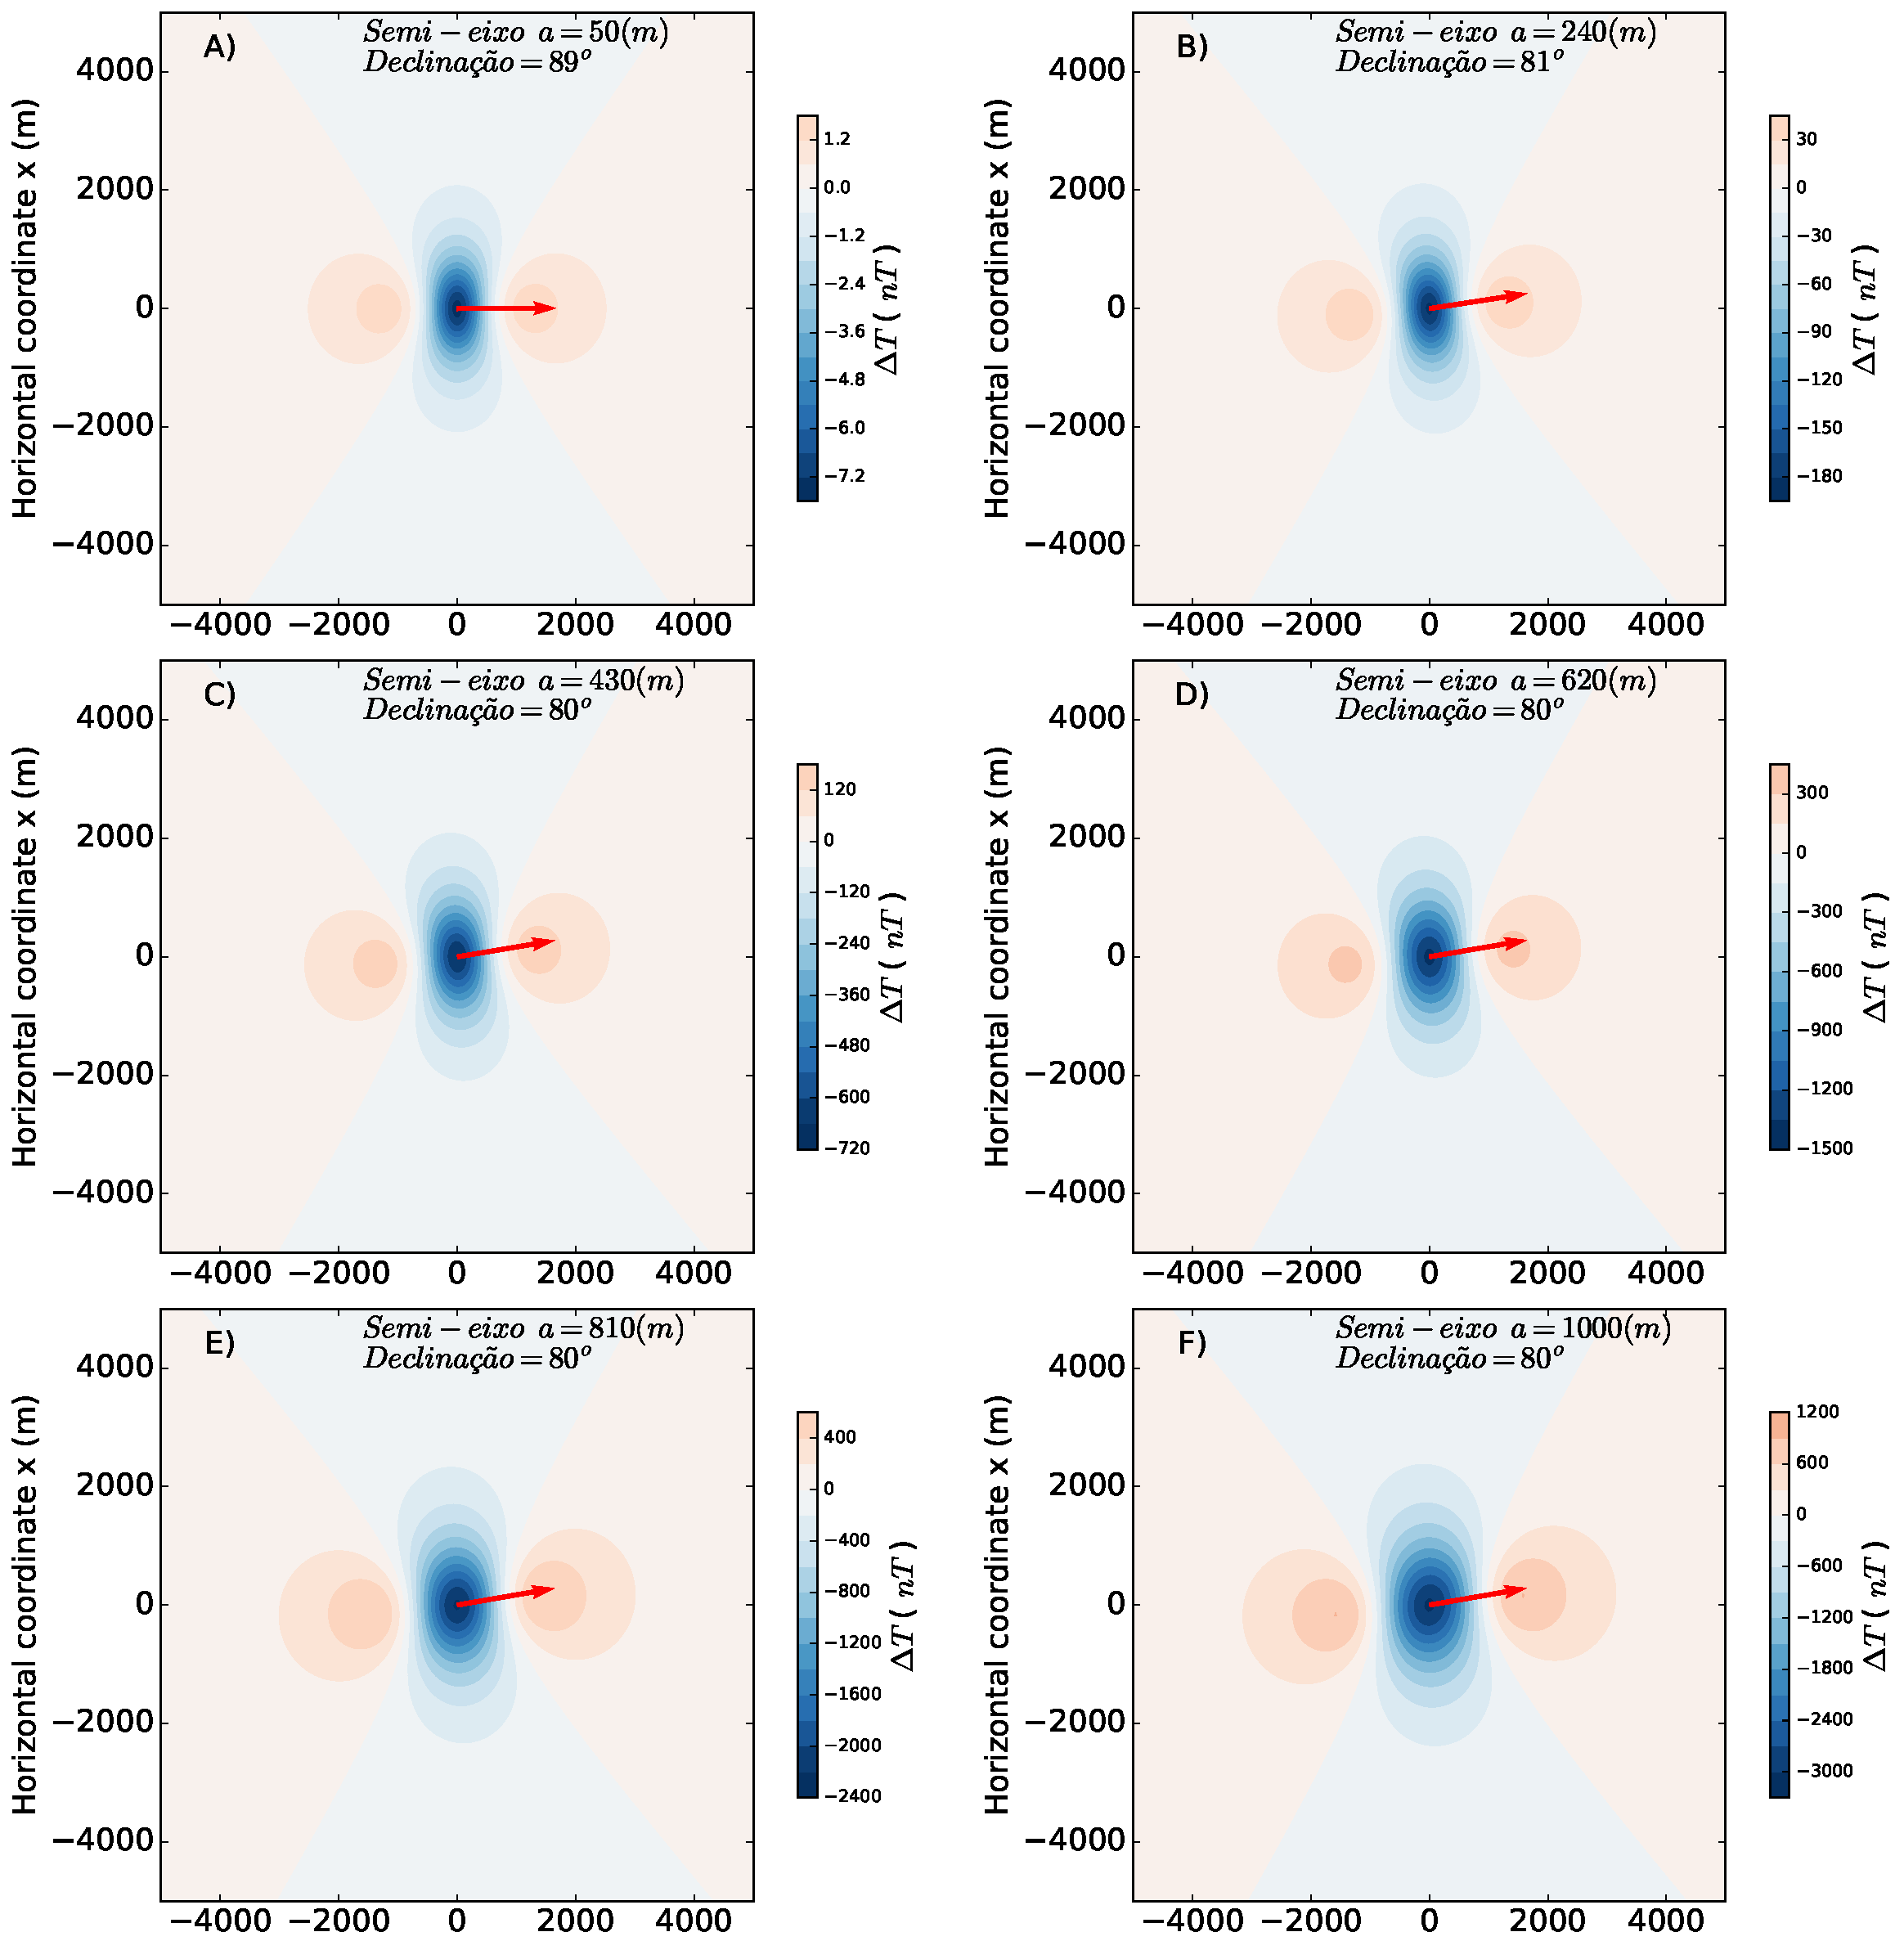
\includegraphics[width=16 cm,height=16 cm]{figures/ellipsoid_shape_iso2}
	\caption[Simulação, da mudança do vetor de magnetização resultante, de um elipsoide triaxial com o aumento do semi-eixo maior.]{Simulação, da mudança do vetor de magnetização resultante, de um elipsoide triaxial com o aumento do semi-eixo maior. O elipsoide está imerso em um campo externo constante de declinação $90^o$, possui susceptibilidade constante e direcionado com um azimute de $80^o$. Ao longo da sequência das figuras, seu semi-eixo maior aumenta de proporção em relação aos demais (variando entre 50 e 3000 m.). Nota-se a tendência do vetor de magnetização resultante (seta em vermelho) em se alinhar com o semi-eixo maior. Diferente da figura anterior, houve pouca mudança na declinação devido ao alinhamento do elipsoide com a campo externo.}
	\label{fig:ellipsoid_shape_iso80}
\end{figure}